\chapter{Middle English (1150--1500)}\label{ME}
\largerpage
\section{History and context}

Conveniently, the Middle English period maps quite neatly onto what is called the (High and Late) Middle Ages in European history. This is popularly known as the age of knights, castles and chivalry. More prosaically, it's also a period of growing populations, booming trade, and (during the Late Middle Ages) terrible catastrophes such as the Black Death.\is{Black Death} As we will see in this chapter, Middle English is also a period typically seen as a transition\is{transition problem} during which the English language underwent some of its most major changes. While the earliest Middle English texts can seem incomprehensible without training, texts from the end of the period look a lot more familiar to most readers.

\subsection{Dividing lines}

\begin{wrapfigure}{r}{0.385\textwidth}
    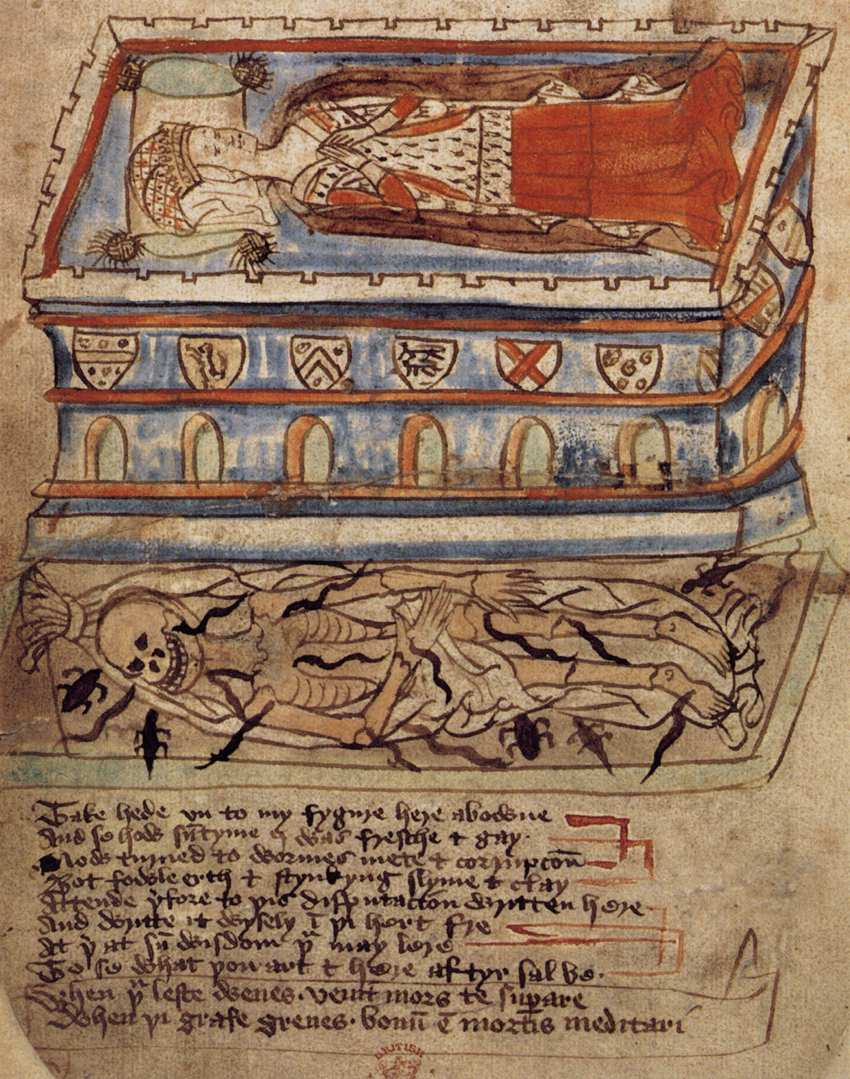
\includegraphics[scale=0.655]{chapters/img/Transitory_tomb_-_1435-40.jpg}
    \caption{An illuminated folio from British Library Additional manuscript\is{manuscripts} 37049, f. 32v}
    \label{fig:ME_transitory}
\end{wrapfigure}

The dividing line between Middle English and Early Modern English is the year 1500. Like all dividing lines, it's arbitrary: people didn't wake up on New Year's Day 1500 speaking a completely different language. Still, 1500 is a relatively good dividing line because of two major events.

The first is Caxton's\ia{Caxton, William} introduction of the printing press\is{printing press} to England in 1476. The consequences of this were discussed in the previous chapter, \sectref{EModE-standardization},\is{standardization} but it's worth reflecting on the situation before printing as well. Without the ability to quickly and automatically reproduce texts, it wasn't at all easy to reach a wide audience, since every single copy had to be made by hand. This was time-consuming and expensive, and it's not surprising that the literacy\is{literacy} rate was extremely low during the Middle English period: even as late as 1451--1500, \citet{BuringhVanZanden2009} estimate that only 5\% of the population was able to read or write. This literacy was also very unevenly distributed across the population, with most of those able to write being part of the (Christian)\is{Christianity} clergy, especially in the first half of the period.\is{literacy} The physical nature and cultural context of our written records from the Middle English period and before is thus very different. We are dealing with handwritten manuscripts,\is{manuscripts} which were extremely rare and valuable objects in their own right, increasingly so the further we go back in time. The introduction of the printing press\is{printing press} towards the end of the Middle English period therefore represents a fairly important event in the history of the language, for several reasons, but also for the historical linguist!\is{standardization}

\largerpage
The second convenient turning point is Christopher Columbus's\ia{Columbus, Christopher} discovery of a reliable sailing route from Europe to the Americas and his voyages there between 1492 and 1501. Columbus himself wasn't English: he was born in Genoa (now part of Italy), and his travels were funded by the Spanish monarchy. He also wasn't the first European to travel to the Americas, but his experiences were instrumental in setting the scene for the colonial expansion of various European states during the Early Modern and Modern periods (see \sectref{EModE-colonial}).\is{colonialism} Before 1500, although some English speakers travelled widely, there were no substantial, stable communities of English-speaking people outside Britain and Ireland. When we talk about the English of the Middle English period and earlier, we are talking about the English spoken and written in England, Scotland, Wales, and Ireland: English had simply not reached the rest of the world during this period.


\begin{varietybox}{Scots}
The West Germanic variety spoken at present in Scotland, today known as \ili{Scots}, has its origins in Northumbrian Old English.\il{Old English, Northumbrian} It's sometimes treated as an English dialect and sometimes as a language in its own right. As you know by now, there are no systematic and accepted linguistic criteria for distinguishing between ``dialects'' and ``languages'': the question is a sociopolitical one. Between 1150 and 1500, the variety was known by its users as \emph{Inglis} (English), just like the English of England; the term \emph{Scottis} (Scottish/Scots) is first recorded in 1494. We can't do justice to the fascinating history of Scots in this book, but see \citet{Jones1997}, \citet{Smith2012}, and \citet[Chapter 3]{Millar2012} if you're interested in finding out more.
\end{varietybox}


\noindent What about the dividing line at the start of the Middle English period, 1150? Here the key event is one that's probably the most famous date in British history: 1066 and the Norman Conquest.\is{Norman Conquest|(}

\subsection{The Norman Conquest and French influence}\label{ME-french}

Any history of Britain will give an account of the events of 1066. In brief, upon the death of King Edward the Confessor,\ia{Edward the Confessor (King)} three rulers scrambled to assert dominance over England: Edward's brother-in-law Harold Godwinson;\ia{Godwinson, Harold} the king of Norway, Harald Hardrada;\ia{Hardrada, Harald} and the duke of Normandy, William the Conqueror.\ia{William the Conqueror} As his name suggests, William the Conqueror was victorious: his army defeated Harold Godwinson's at the Battle of Hastings in October 1066. (Harald Hardrada's forces had been defeated three weeks earlier by Godwinson's at the Battle of Stamford Bridge.)

\begin{figure}
    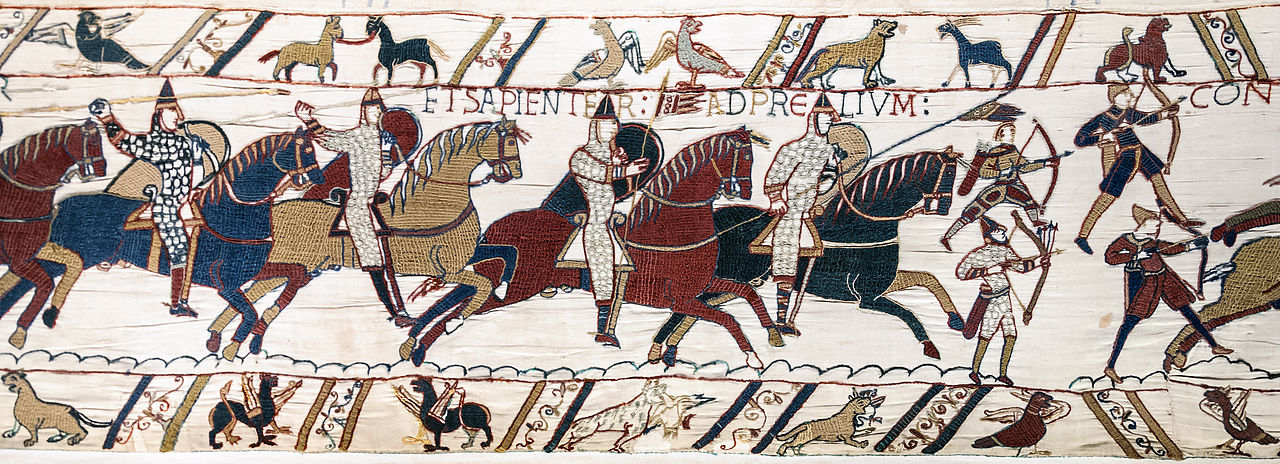
\includegraphics[scale=1.15]{chapters/img/1280px-Bayeux_Tapestry_scene51_Battle_of_Hastings_Norman_knights_and_archers.jpg}
    \caption{Norman knights and archers at Hastings, from the famous Bayeux Tapestry}
    \label{fig:ME_Hastings}
\end{figure}

\noindent It's easy to overplay and essentialize the differences between these three men: Harold the ``Saxon'',\ia{Godwinson, Harold} Harald the ``Norseman'',\ia{Hardrada, Harald} and William the ``Norman''. In reality, they had plenty in common. Godwinson's mother was the Scandinavian Gytha Thorkelsdóttir,\ia{Thorkelsdóttir, Gytha} a noblewoman from Denmark. William\ia{William the Conqueror} was descended from Rollo\ia{Rollo of Normandy} (or Hrólf), a Scandinavian Viking\is{Vikings} leader of the ninth and tenth centuries who eventually settled and established Normandy as a political entity: the terms \emph{Norman} and \emph{Normandy} originated in reference to the northern origins of these settlers. Even Edward the Confessor\ia{Edward the Confessor (King)} was half-Norman through his mother Emma.\ia{Emma of Normandy}

Nevertheless, the linguistic impact of William's conquest was dramatic. Wil\-liam was brought up in Normandy, now part of France, where the dominant language was the Norman dialect of Old French.\il{French, Norman} As part of the conquest, on becoming king, he appointed several of his French-speaking allies to positions of power within England. William\ia{William the Conqueror} himself died in 1087, but his successors for the next four hundred years were monarchs whose ties to France were at least as strong as their ties to England. In particular, the House of Plantagenet held the throne of England from 1154 until the death of Richard III in 1485.\ia{Plantagenet, Richard (King Richard III)} This quite naturally led to \ili{French} -- first Norman French,\il{French, Norman} then Parisian French -- becoming the language with the most overt \glossterm{gl-prestige}{prestige}\is{prestige} in England, and being used for a wide range of political, literary and other functions. Among the literate\is{literacy} minority, in particular, there was widespread English-\ili{French}-\ili{Latin} trilingualism \citep[§11.2]{Durkin2014}. Throughout this chapter we'll see evidence of \ili{French} influence on Middle English, especially as regards the lexicon. This situation certainly had important effects on the vocabulary of the language, but also on some of its structural properties.


\begin{varietybox}{Anglo-Norman}
\il{French, Norman}\il{French, Anglo-Norman}
The variety of Norman \ili{French} spoken in Britain during the Middle English period is known as Anglo-Norman, and rapidly developed its own linguistic features, distinct from those found in Normandy itself. Introduced as the language of a relatively small elite, Anglo-Norman was never ubiquitous among the population of England. The dominant view until recently was that Anglo-Norman died out in England fairly rapidly from about 1160 onwards, but \citet{Ingham2012}, following \citet{Rothwell2001}, makes a powerful case that the language was still being transmitted and learned by children until at least the beginning of the fifteenth century, and that Middle English and Anglo-Norman continued to influence each other as living languages throughout.\is{Norman Conquest|)}
\end{varietybox}


\subsection{Middle English texts}\label{ME-text-transmission}

The Middle English period has been described as having ``by far the greatest diversity in written language of any period before or since'' \citep[156]{Milroy1992}. Just take a look at the text samples at the end of this chapter! Certainly the limited Old English records that have survived to us, and the more-or-less \glossterm{gl-standardization}{standardized}\is{standardization} written language of the period 1500--1900, are more homogeneous. Only the present day, with its superdiversity of Englishes around the world, might be said to have a better claim to this title.

Nevertheless, the Middle English textual records are skewed and limited in certain important ways. For a start, as we've seen, Middle English is exclusively a language of Britain and Ireland. The majority of texts that have come down to us are also written by men rather than women. On the other hand, the first named female authors to enjoy a wide reception also date from this period: the mystics \iai{Julian of Norwich}, whose \emph{Revelations of Divine Love} was written in the 14th century, and Margery Kempe,\ia{Kempe, Margery} who wrote her semi-autobiographical \emph{Book of Margery Kempe} in the early 15th century. We also have letters written by the Paston family of Norfolk, both men and women, from the 15th century -- though we can't be sure to what extent these documents reflect women's language, as the scribes\is{scribes} who were employed to write the letters were all male.\footnote{See \citet{HernandezCampoyCondeSilvestre2004} and \citet{Bergs2011} for studies investigating the Paston letters from a sociolinguistic\is{sociolinguistics} perspective.} This highlights another important limitation: basically all Middle English writers were part of the church, the nobility, or both.

The early and late parts of the Middle English period also differ in terms of what texts have come down to us. Traditional scholarship has often stated (or at least implied) that English as a written language died out entirely after the Norman Conquest,\is{Norman Conquest} later rising phoenix-like from the flames during the 13th and 14th centuries. Under this view, the transition\is{transition problem} from Old to Middle English is very abrupt. However, \citet[Chapter 5]{Treharne2012} shows convincingly that this interpretation is not justified: hundreds of texts were produced in English during this early period, and these are catalogued online in \citet{DaRoldEtal2010}. The disregard shown to these texts by scholarship until relatively recently may be due to the fact that these were generally not brand-new literary texts, instead building on and reworking earlier Old English material. This also means that it is difficult to know to what extent these texts reflect the spoken language of the period. In the 12th century, however, a few texts like the Peterborough Chronicle, a historical record kept by monks in the east of England, and the \emph{Ormulum},\ia{Orm} another East Midlands text dealing with the interpretation of the Bible (and written in a unique phonetically-inspired orthography),\is{orthography} give us an indication of some of the changes that the language had undergone.

The texts aren't evenly distributed geographically, especially during the early part of the period.\is{regional variation} For the 12th century, most of our localizable texts are from the East Midlands.\il{Middle English, East Midlands} In the 13th century this shifts, with a proliferation of West Midlands\il{Middle English, West Midlands} texts attested, such as Layamon's\ia{Layamon} \emph{Brut}, a poem\is{poetry} about the history of Britain. The 14th and 15th centuries are better attested, and our first texts from north of the Humber estuary date from this later part of the period. This is also when the texts emerge that have been most intensively studied as works of literature: Arthurian romances such as \emph{Sir Gawain and the Green Knight}, and poetry\is{poetry} by such writers as William Langland,\ia{Langland, William} John Gower,\ia{Gower, John} and Geoffrey Chaucer.\ia{Chaucer, Geoffrey} Figure \ref{fig:ME_locations} gives an overview of some important texts and writers and where they were from (or where they wrote).

\begin{figure}

     \begin{tikzpicture}
        \node[align=center] (map) at (6,4)
        {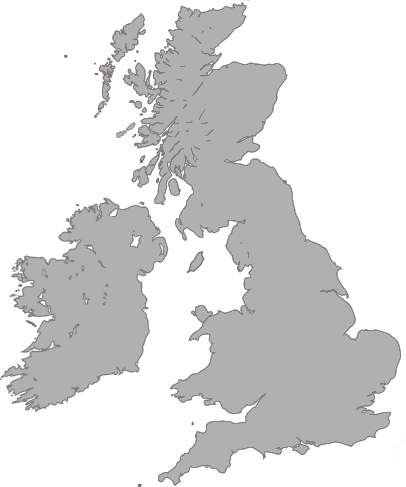
\includegraphics[width=.6\textwidth]{chapters/img/blank-uk.png}};
        \filldraw[fill=lsLightGreen,draw=black] (0.8,0) rectangle (3.7,2);
        \node[align=center] (WestSaxon) at (2.25,1) {\textbf{Southern}\\John of Trevisa\\Caxton\\Chaucer};
        \filldraw[fill=lsRed,draw=black] (0.25,3.2) rectangle (1.75,4.6);
        \node[align=center] (Irish) at (1,3.9) {Kildare\\Poems};
        \filldraw[fill=lsMidBlue,draw=black] (0.5,5.9) rectangle (3.6,7.5);
        \node[align=center] (WMid) at (2.05,6.7) {\textbf{West Midlands}\\Sir Gawain\\Ancrene Wisse};
        \filldraw[fill=lsLightWine,draw=black] (10,0.7) rectangle (12,2.3);
        \node[align=center] (Kentish) at (11,1.5) {\textbf{Kentish}\\Ayenbite\\of Inwyt};
        \filldraw[fill=lsMidOrange,draw=black] (9.1,3) rectangle (11.9,3.6);
        \node[align=center] (Norfolk) at (10.5,3.3) {Paston Letters};
        \filldraw[fill=lsYellow,draw=black] (8.5,6.2) rectangle (11,7.8);
        \node[align=center] (Northern) at (9.75,7) {\textbf{Northern}\\Richard Rolle\\Cursor Mundi};
        \filldraw[fill=lsMidGreen,draw=black] (8.8,4.5) rectangle (11.6,5.5);
        \node[align=center] (EMid) at (10.2,5) {\textbf{East Midlands}\\Ormulum};
        \draw[->] (10.5,3) -- (9.3,2.3);%Paston
        \draw[->] (10.1,1.5) -- (9.2,0.77);%Ayenbite
        \node[align=center] (Canterbury) at (10,0.5) {\footnotesize{Canterbury}};
        \draw[->] (8.6,7) -- (7.9,3.1);%Rolle
        \draw[->] (9.3,4.8) -- (8.3,2.2);%Ormulum
        \draw[->] (8.7,6.4) -- (8.2,3.4);%Cursor Mundi
        \node[align=center] (York) at (7.65,3.5) {\footnotesize{York}};
        \draw[->] (3.5,1.15) -- (7.1,1.2);%Trevisa
        \draw[->] (3.1,0.6) -- (8.3,1);%Caxton/Chaucer
        \node[align=center] (London) at (8.3,1.2) {\footnotesize{London}};
        \draw[->] (3,6.7) -- (7.3,2.6);%Gawain
        \draw[->] (2.9,6.05) -- (7,2);%Ancrene
        \draw[->] (1.75,3.9) -- (4.5,2.7);%Kildare
     \end{tikzpicture}
     \caption{Some key texts and authors during the Middle English period}
     \label{fig:ME_locations}
\end{figure}



\begin{peoplebox}{Chaucer}
\ia{Chaucer, Geoffrey}
Geoffrey Chaucer (c. 1343--1400) is one of the most famous English-language writers of all time. Born into a family of merchants, he travelled Europe as a young adult, and later spent twelve years working as a high-ranking customs official in London. Best known for his literary output, especially the \emph{Canterbury Tales}, he also produced philosophical and astronomical texts. Like other key figures of the period (e.g. Gower,\ia{Gower, John} Caxton),\ia{Caxton, William} Chaucer was multilingual,\is{multilingualism} and his writings show him expertly navigating the space between English, \ili{French} and \ili{Latin} \citep{Davidson2010,Hsy2013}. An introduction to Chaucer's life and works can be found in \citet{Minnis2014}, and the recent biography by \citet{Turner2019} foregrounds his European travels.
\end{peoplebox}


\noindent For many readers, Middle English is the period when the texts really start to feel like they're written in a different language. On the other hand, it's not quite as alien-looking as Old English is, as we will see in \chapref{OE}. Early Middle English texts in particular are difficult to understand if you're not aware of the peculiarities of morphology and syntax in this language stage, closer to Old English in its appearance. Don't worry, though: in this and the following chapter we'll be including details that will help you to make sense of what you see.

\begin{figure}
    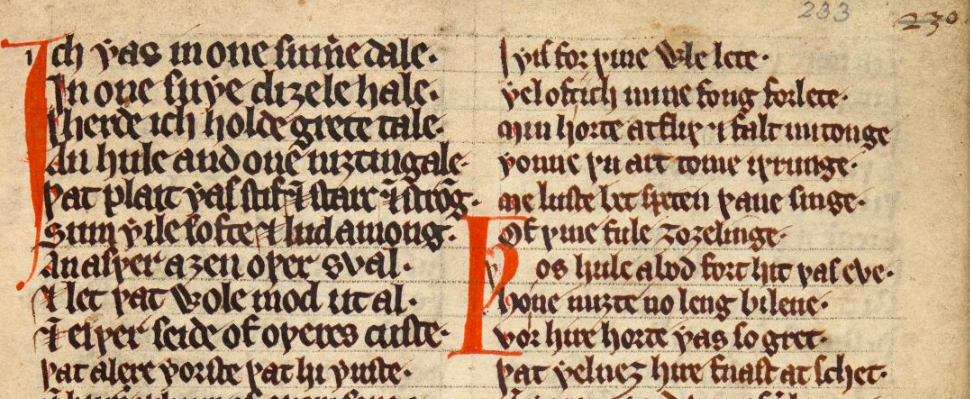
\includegraphics[scale=0.36]{chapters/img/OwlNightingale.png}
    \caption{An illuminated folio from the British Library from Cotton MS Caligula A IX, ff. 322 r., showing the beginning of \textit{The Owl and the Nightingale}}
    \label{fig:owl-folio}
\end{figure}

To keep things relatively simple, in this introductory chapter we'll present you with what could be seen as Chaucer's\ia{Chaucer, Geoffrey} English, since that's the type of Middle English you'll most likely encounter in your literature classes. This is not to imply, however, that Chaucer's\ia{Chaucer, Geoffrey} English is either the only type of Middle English or a variety of Middle English more prestigious than other Middle English varieties -- neither is the case. We have evidence of Middle English varieties used from the far north to the far south of England, from the west coast to the east coast, and spanning a period of four hundred years -- though not all areas or centuries are equally well represented.\is{regional variation} If you want to get your hands dirty and dive into Middle English in all its glorious diversity, we recommend the Linguistic Atlases of Late Middle English (LALME) and Early Middle English (LAEME), both available online for anyone to use.\footnote{LALME: \url{http://www.amc.lel.ed.ac.uk/amc-projects-hub/project/elalme/}. LAEME: \url{http://www.amc.lel.ed.ac.uk/amc-projects-hub/project/laeme/}.}

\section{Sounds}
In this section, we'll first provide a general overview of the phonological system of Middle English. We will also introduce you to some graphical features of Middle English to be aware of when approaching texts. Finally, we will take you through the main sound changes of this period as well. As we will see, Middle English is full of variation on every corner, and this variation stands out already at the first glance at most texts written in the language of the time, for Middle English can indeed be considered the period associated with the least standardized\is{standardization} spelling\is{orthography} in the entire history of the English language as used in Britain. This is not surprising considering the sociocultural changes happening during this period. Read on to discover more!

\subsection{General properties of Middle English phonology}
Looking at the phonological system of Middle English, we'll notice several differences in contrast to the phonological system of standard Present Day English varieties:
\begin{itemize}
    \item there is no \glossterm{gl-phoneme}{phoneme} /ŋ/; the sound [ŋ] does exist, but only as an \glossterm{gl-allophone}{allophone} of /n/
    \item there is no phoneme /ʒ/
    \item there is an additional phoneme, the velar fricative /x/ (still found in Scottish English\il{English, Scottish} in Present Day English)
    \item the vowels\is{vowels} look rather different from those found in Present Day English as well as Early Modern English
    \subitem -- we distinguish short and long vowels\is{vowels} in stressed syllables
    \subitem -- unstressed syllables carried important morphosyntactic functions\is{stress shift}
    \subitem -- we find diphthongs\is{vowels} not necessarily like those in Present Day English
\end{itemize}

\begin{figure}[t]
  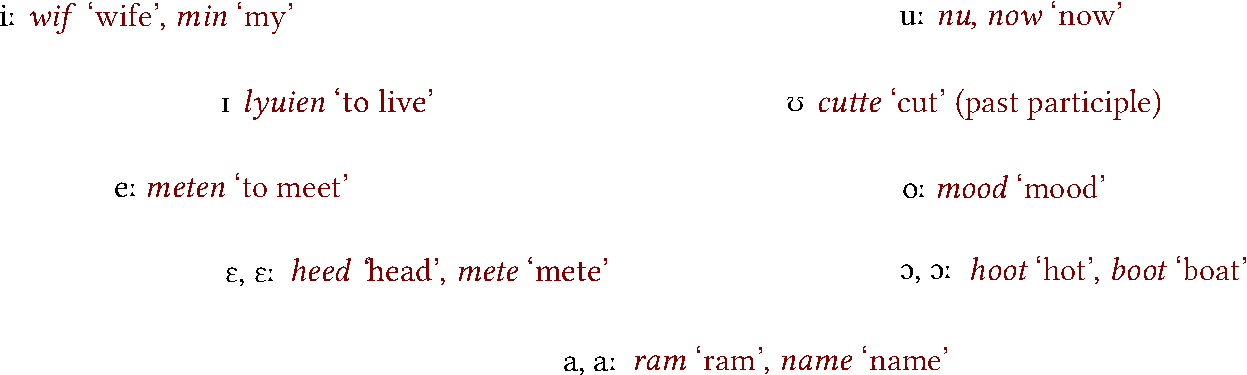
\includegraphics[width=\textwidth]{chapters/img/MEmonophthongs.pdf}
  \caption{Chaucerian Middle English monophthongs, based on \citet[48]{HorobinSmith2002}}
  \label{fig:MEmonophthongs}
\end{figure}

% \noindent
Middle English monophthongs are shown in Figure \ref{fig:MEmonophthongs}. In addition to these twelve monophthongs, there were also five diphthongs: /aɪ/ \textit{day}, /ɔɪ/ \textit{joye}, /aʊ/ \textit{saugh} `saw', /ɔʊ/ \textit{knowe} `to know', and /ɪʊ/ \textit{newe} `new'. But this is not where the differences end, as we shall see in what follows in this section. However, we need to learn a little bit about some of the aspects of Middle English spelling first.

\subsection{Graphical features to look out for}\label{ME-graphical}\is{manuscripts|(}
When dealing with texts written in Middle English, it's important to be aware of some graphical\is{orthography|(} differences between Middle English and Present Day English which may startle you at first. To begin with, Middle English is typically seen as \textit{the} period of spelling and phonetic variation \citep[224]{Strang1970} in the history of the English language. For instance, \citet[33]{HorobinSmith2002} mention that the Present Day English word \textit{though} is attested in more than 500 spelling variants between the years 1350 and 1450. We find a considerable degree of variation across different regions,\is{regional variation} but we also find variation across individual scribes\is{scribes} -- irrespective of the region. In addition, even a single scribe frequently shows variation: not just across different manuscripts but also within a single one. To illustrate the point, let's have a look at how the word \textit{when} is spelt in the Cotton Caligula manuscript version of \textit{The Owl and the Nightingale}. In line 620, we find <wan>, alongside variants such as <wane> (line 420), <wone> (line 687), <wanne> (line 1446), <won> (line 324), <wonne> (line 38); and in line 1566 we find <hwon>, and yet other variants can be seen in the same manuscript: <hwanne> in line 1244; <hwan> in line 1537, <hwon> in line 1566.


\begin{sourcebox}{Books were expensive}

If you're reading this book, it's rather likely you come from or have found yourself in a society where a range of individuals from different social groups can produce texts of various types online or offline via digital software. Chances then also are that it's not a problem to grab a piece of paper and scribble down whatever your heart desires. This was far from being the case in the Middle English period. Paper was to arrive in Britain only in the 15th century \citep[9]{HorobinSmith2002}. Prior to this, parchment was used for writing: scribes\is{scribes} used animal skin to pass down what was considered worth the effort and the materials. The costs associated with obtaining enough parchment formed just one rather small part associated with the book making process \citep{Overty2008}.
\end{sourcebox}


\noindent Considering how much spelling variation there is in Middle English texts, we can't discuss all the spelling variation that awaits anyone who intends to read texts in Middle English. However, here are at least some general, more obvious graphical differences between Present Day English and Middle English. First, in Middle English we still find a letter called \glossterm{gl-thorn}{thorn},\is{thorn} which looks like this: <þ>.\footnote{You may have seen this unfamiliar letter already in the previous chapter if you read the text sample from Anne Askew's \textit{Examinations}.} This letter was ultimately replaced by the Present Day English <th>, but we find it frequently both in Middle English and Old English texts (see \chapref{prehistory}, \sectref{prehistory-runes}, for more details). Just like the Present Day English <th>, thorn\is{thorn} could be used to represent either the voiced dental fricative /ð/ or the voiceless dental fricative /θ/. We also encounter a letter known as \glossterm{gl-yogh}{yogh}\is{yogh} /jɒx/, which is written this way: <ȝ>. This letter was used primarily for the sounds /j/ and /x/ (the latter being a voiceless velar fricative).

We should also comment on how, under the influence of the Norman\il{French, Norman} scribal\is{scribes} traditions, the sound /u/ came to be spelt with <ou>. If you speak or learn \ili{French}, this will make a lot of sense to you, as French textbooks often tell the learner that <ou> is to be pronounced as /u/. As mentioned in \chapref{EModE} (\sectref{EModE-GVS}), in some Present Day English dialects in the north of Britain\il{English, Northern England}\il{English, Scottish} words such as \textit{mouth} can be pronounced with a vowel resembling /u/, which is the vowel\is{vowels} we also find in these words in Middle English (and Old English).\is{regional variation} This is reflected by the <ou> spelling in such words, coexisting with an older simple <u>, as in <mouth> and <muð> for \textit{mouth} /muːθ/, and <hous> and <hus> for \textit{house} /huːs/.


\begin{sourcebox}{Ye Olde Shop}

Where does the phrase \textit{ye olde shop} come from? The strangely looking letter <y> in phrases of this type has descended from the letter \glossterm{gl-thorn}{thorn},\is{thorn} <þ>. Thorn could be hand-written in a number of ways. Think for instance of how you write a word such as \textit{the}: is it always shaped in exactly the same way and does your handwriting match that of others? Once we start looking at manuscripts more closely, we find a range of shapes that thorn came in. One of the shapes found could be interpreted as the letter <y> instead. This ambiguity opened the window to reinterpreting one letter (thorn) with another (<y>). So, the standard Present Day English version of the definite article, <the>,\is{articles} represents a substitution of thorn with the digraph <th>, whereas the version spelt as <ye> represents a substitution of thorn with the letter <y>. See Figure \ref{fig:thorn} if intrigued.\is{orthography|)}
\end{sourcebox}


\begin{figure}[t]
    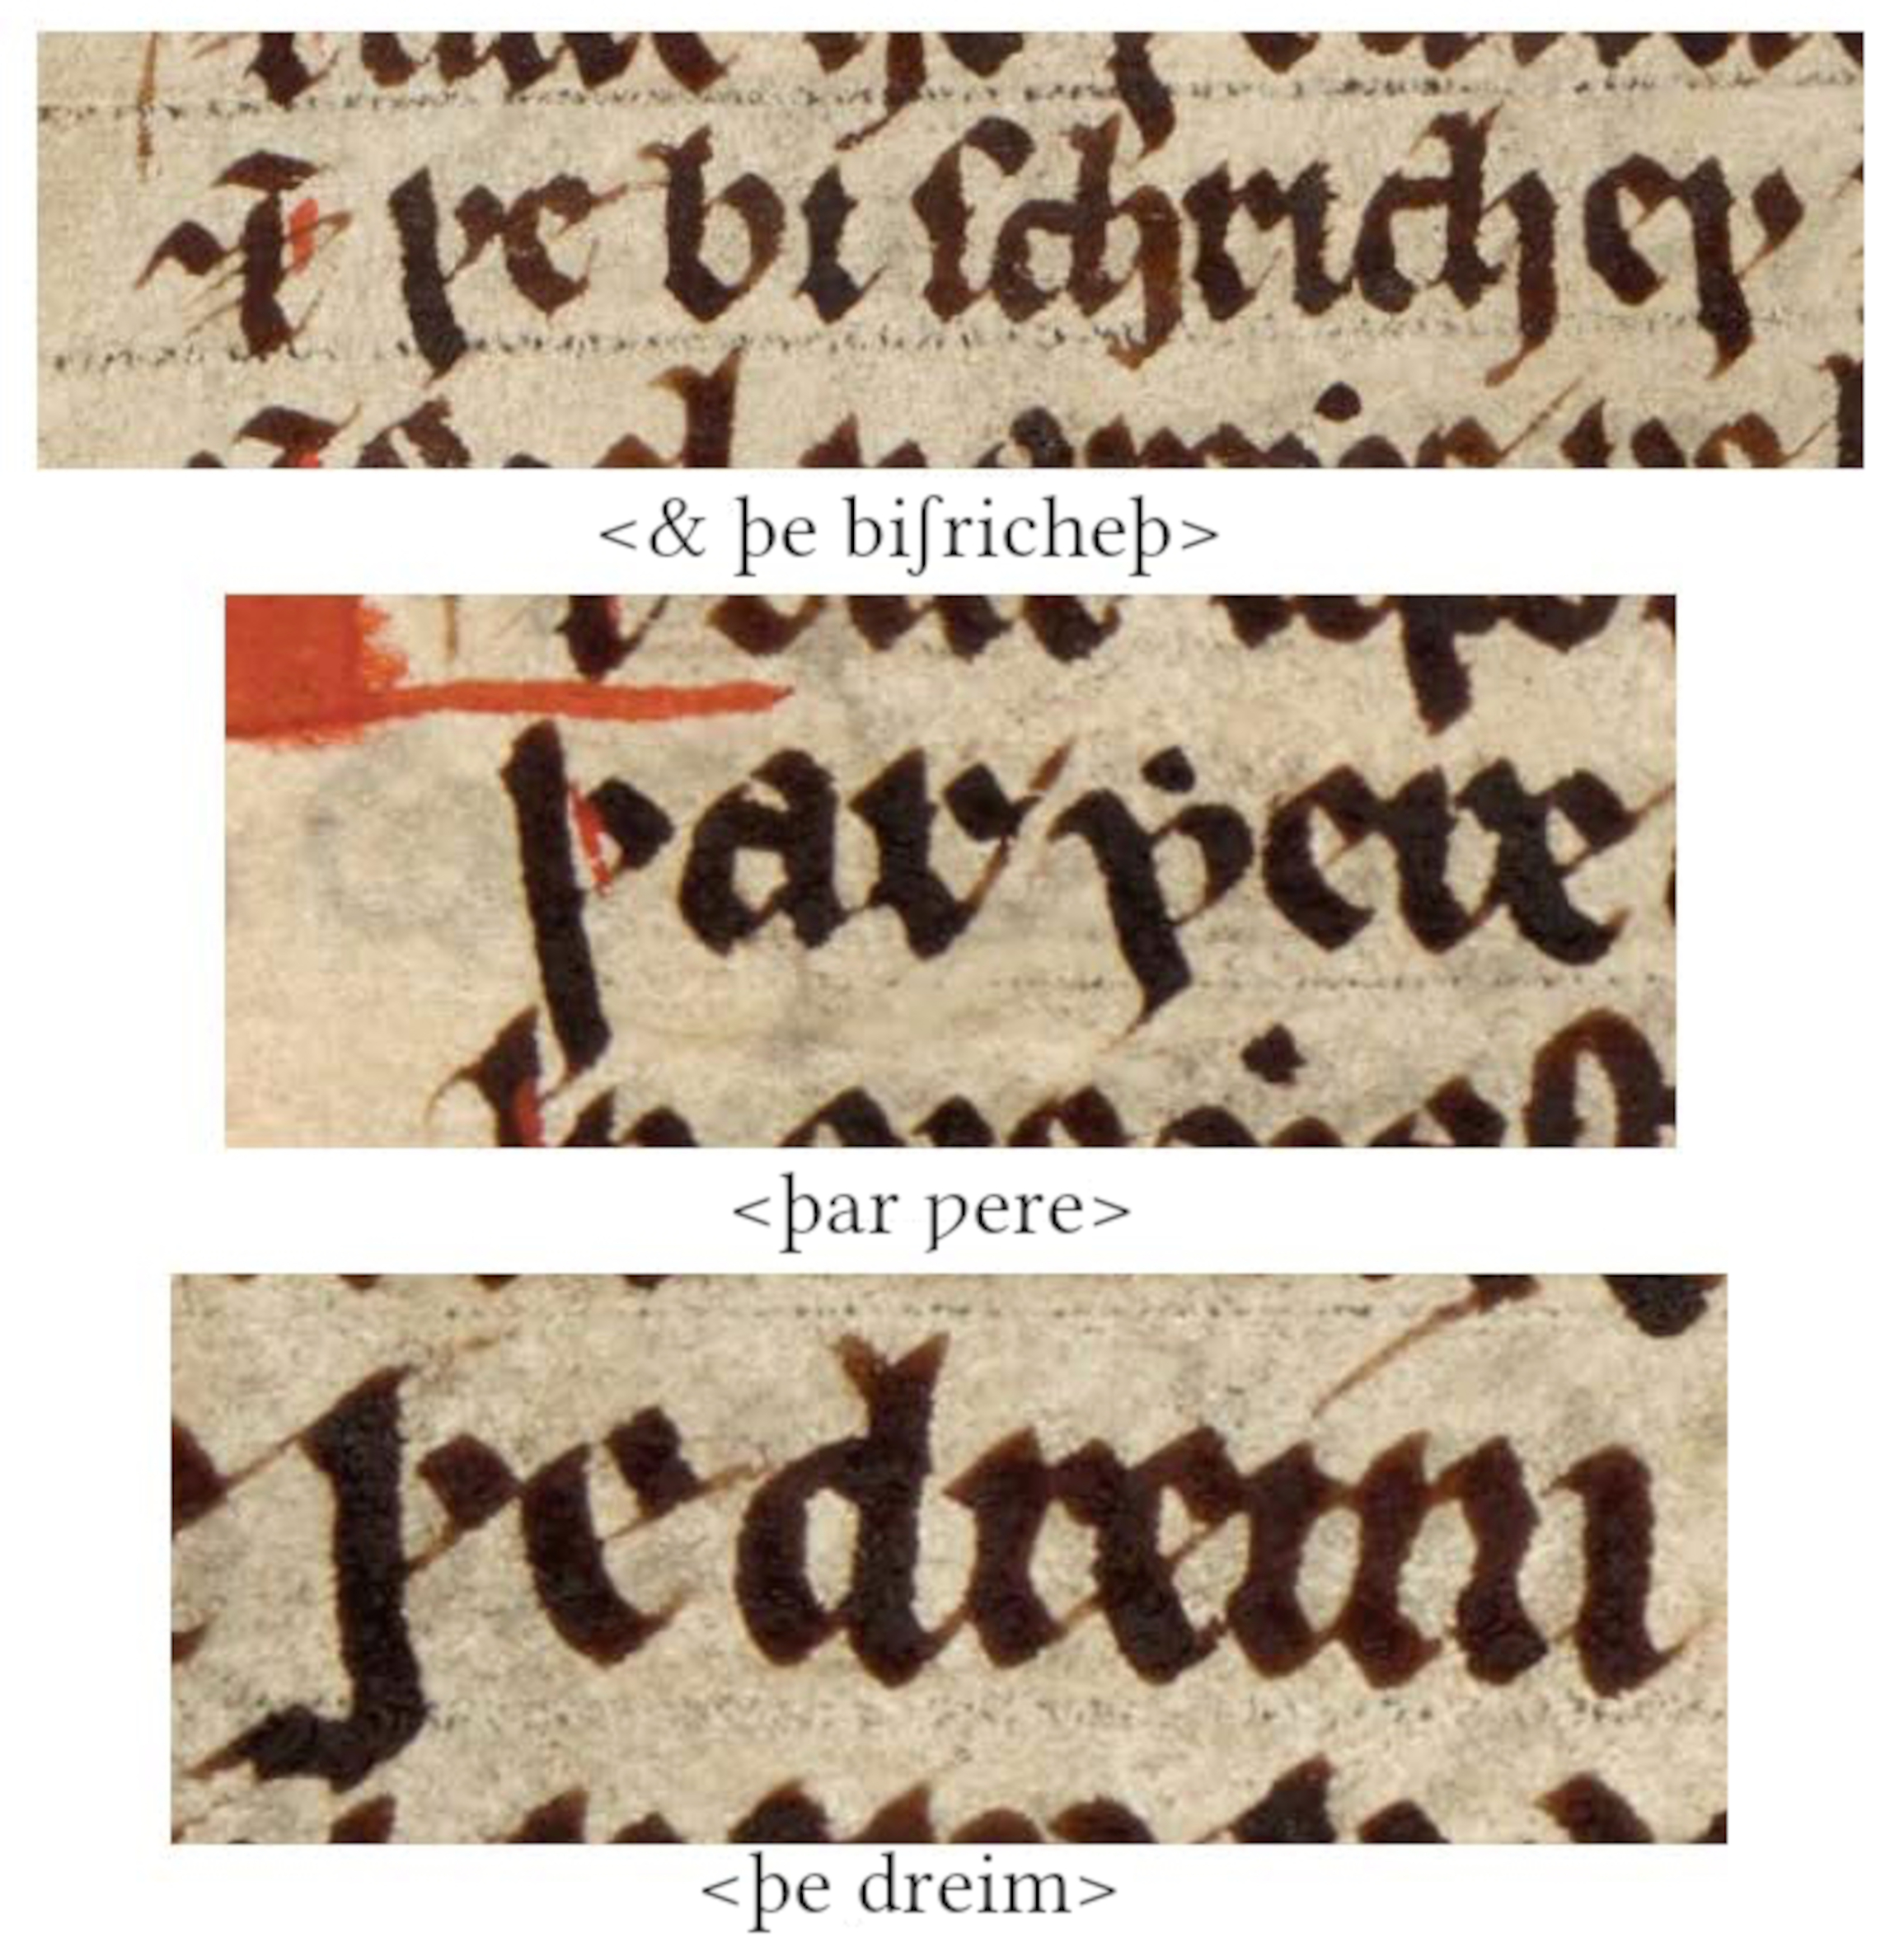
\includegraphics[height=0.5\textheight]{chapters/img/Ch5_Thorn_mod.jpg}
    \caption{An illuminated folio from the British Library from Cotton MS Caligula A IX, ff. 322 r., showing three close-ups\is{thorn}\is{manuscripts|)}}
    \label{fig:thorn}
\end{figure}

\subsection{/h/-clusters and /h/-dropping}\label{ME-hdrop}\is{/h/-dropping|(}\is{clusters (consonant)|(}
Remember\is{consonants|(} instances of words such as \textit{house} being pronounced variably either as /haʊs/ or /aʊs/ from \chapref{LModE}? Indeed, we've already seen the phenomenon of \glossterm{gl-hdrop}{/h/-dropping} and the social stigma attached to it in LModE and Present Day English in \sectref{LModE-hdrop}. This phenomenon is attested already in Old English, but crucially primarily in pronouns\is{pronouns} and unstressed words. /h/-dropping in unstressed syllables is common for all varieties of English today, standard and non-standard, and is not stigmatized \citep[104]{Minkova2014}. On the other hand, omission of <h> in words such as \textit{house}, i.e. words that contain at least one syllable with primary stress, is sporadic in Old English: it is only in Middle English when initial /h/ in stressed syllables is attested more frequently.\is{frequency} In this context, it's interesting that \ili{French} loans\is{borrowings} which in writing started with an initial <h> did not contain an /h/ in pronunciation in the source language -- this may have only contributed to an overall confusion as to whether one should or should not pronounce an /h/ in words such as \textit{honour} (of Romance origin) or \textit{house} (of Germanic origin).

/h/-dropping is not the only feature that's of relevance to the changes linked to this consonant in Middle English. What we variably find in Middle English is also the presence of /h/ in clusters that no longer survive in Present Day English: /hl/, /hr/, and /hn/; and also one cluster which has survived in some Present Day English dialects: /hw/ or /ʍ/. Similarly to /h/-dropping, we also start seeing the loss of /h/ in these clusters in Middle English. We'll see that Old English had these four clusters by default. Although traces of this cluster reduction do show up in Old English, the process properly kicks in only in Middle English. This cluster reduction change had swooshed through these clusters by the end of Middle English, simplifying them to /l/, /r/,\is{/r/} and /n/ and giving us \textit{lofe} for the older \textit{hlaf} `loaf', \textit{raven} for the older \textit{hræfn} `raven', and \textit{nut} for the older \textit{hnut} `nut'. This cluster simplification process has never really reached completion in the case of /w/ and /ʍ/. And just like in Present Day English, where we find variation between /w/ and /ʍ/, as in /wɛɪlz/ vs. /ʍɛɪlz/ \textit{whales} (see \chapref{introduction}), in Middle English we also find variable forms reflected in the spelling, even within a single manuscript.\is{manuscripts} These cluster simplifications lead to a language which is phonologically closer to Present Day English.\is{/h/-dropping|)}


\begin{soundbox}{\textit{gnats} /gnats/ and \textit{knives} /kniːvəs/}

In Middle English, the word-initial <gn> and <kn> were pronounced as consonantal clusters: /gn/ and /kn/, respectively! This is still preserved in the Present Day English spelling,\is{orthography} although these clusters were simplified to /n/ over the course of time.\is{consonants|)}\is{clusters (consonant)|)}
\end{soundbox}


\subsection{Reduction of vowels in unstressed syllables}\label{ME-reduction}\is{vowel reduction|(}
Some\is{vowels|(} of the spelling\is{orthography} and phonological variation typical of the Middle English period is related to the vowels found in unstressed syllables. Look at the following spelling\is{orthography} variants of the same words (OED; \glossterm{gl-sv}{s.v.} `book, n.', `feel, v.', and `see, v.'):

\begin{exe}
    \ex `to see': <sien>, <sie>, <sy>
    \ex `books': <bowkes>, <buckys>
    \ex `felt': <felede>, <felide>, <feled>, <felid>, <feld>
\end{exe}

\noindent These are just a couple of representative examples taken from the OED. However, these variants do not merely reflect orthographic\is{orthography} variation. Rather, this variation is representative of phonological variation as well. Thus, a form such as <sien> indicates that the nasal consonant\is{consonants} /n/ was part of the infinitive form of the verb, but a form such as <sie> indicates a lack of this consonant.\is{consonants} Next, if we contrast <sie> and <sy>, we could suggest that the former may contain a schwa, i.e. be pronounced as /siːə/ rather than /siː/. 

These instances of vowel reduction are attested in some dialects of Old English already, but the process takes up speed as we transition into and throughout the Middle English period. As we'll see in \sectref{ME-verbs} and \sectref{OE-case}, this vowel reduction process was to have massive consequences for the morphological system of the language.


\begin{sourcebox}{Middle English poetry: to schwa or not to schwa?}
\is{poetry}
Words ending in <e> in Middle English manuscripts\is{manuscripts} feature in many hot debates over whether these <e>s were realized as schwas or nothing at all. This seemingly innocent issue has implications for our understanding of the metrical system of the poetic works at hand, since the numbers of syllables are at stake. If you'd like to know more, we refer you to \citet{Duffell2000} as a sample case study.\is{vowel reduction|)}
\end{sourcebox}


\subsection{A note on vowel lengthening and shortening}\label{ME-lengthening}\is{vowel shortening|(}\is{vowel lengthening|(}
Have you ever wondered how come the word pairs below show the irregularities\is{irregularities} they do? At least two consonants\is{consonants} in each pair indicate that the two words on each line are related: \textit{keep} and \textit{kept} both contain the letters <k> and <p>, corresponding to the sounds /k/ and /p/. And the spelling\is{orthography} representing the vowel in each pair is not too dissimilar either: e.g. <ee> vs. <e>. In Present Day English, these pairs contain different vowel phonemes, and that's what makes them irregular.\is{irregularities} So how did these vowel differences come about?

\begin{multicols}{2}
\begin{itemize}
    \item \textit{keep} \textasciitilde \textit{kept}
    \item \textit{leave} \textasciitilde \textit{left}
    \item \textit{lead} \textasciitilde \textit{led}
    \item \textit{speed} \textasciitilde \textit{sped}
    \item \textit{breed} \textasciitilde \textit{bred}
    \item \textit{breathe} \textasciitilde \textit{breath}
    \item \textit{steal} \textasciitilde \textit{stealth}
    \item \textit{divine} \textasciitilde \textit{divinity}
    \item \textit{child} \textasciitilde \textit{children}
\end{itemize}
\end{multicols}

\noindent In \chapref{EModE}, we've seen the effects of the Great Vowel Shift\is{Great Vowel Shift} on the long vowels of the language (\sectref{EModE-GVS}), which were thereby qualitatively transformed (e.g. Middle English /eː/ became Early Modern English /iː/). Sticking to the \textit{keep} \textasciitilde \textit{kept} pair, in Present Day English \textit{keep} contains an /iː/, whereas \textit{kept} contains an /ɛ/. What happened here is that the vowel in \textit{keep} is long, and was long also in Middle English; so as a long vowel, it underwent the Great Vowel Shift: /keːp/ > /kiːp/. But the vowel in \textit{kept} was short and thus remained unaffected. This vowel length difference, combined with the effect of the Great Vowel Shift,\is{Great Vowel Shift} explains why \emph{keep} shows /i:/ whereas \emph{kept} shows /ɛ/, i.e. a different vowel quality as well as quantity.

In Middle English, before the Great Vowel Shift\is{Great Vowel Shift} kicked in, most pairs such as \emph{keep} and \emph{kept} didn't differ in vowel quality, but all of these pairs did differ in vowel quantity, i.e. whether the vowel was long or short. It's really crucial to remember that only long vowels underwent the Great Vowel\is{Great Vowel Shift} Shift.\footnote{And if you wonder about the difference between the Present Day English [ɛ] and the Middle English [e], this is a phonetic one. [e] has been lowering\is{vowel lowering} in many varieties. See our discussion of vowel shifts taking place in Present Day English in \sectref{NC-shifts}.\is{Northern Cities Shift}}

As shown in Figure \ref{fig:MEmonophthongs} above, vowel length presented a dimension of vowel contrasts that could have implications for the lexical meaning of a word so that if for example the word \textit{name} /naːm(ə)/ `name' was pronounced with a short vowel, this would result in a different word, \textit{nam} /nam/ `took' (past tense, singular). Several processes related to vowel length took place in Middle English, known under the rather complex names of lengthening before voiced homorganic consonant\is{consonants} groups, shortening before non-homorganic consonant\is{consonants} groups, open syllable lengthening, and trisyllabic shortening. Don't worry, we've given you enough Middle English phonology at this stage and won't discuss these processes individually (though much ink has been spilt debating these four fascinating and intricate processes; see \citealp[156--159]{MillHay2018} and \citealp[§7.5]{Minkova2014}).

It is useful, however, to know that there were a number of shortening and lengthening processes operating in Middle English, which resulted in the irregular\is{irregularities} pairs given above. Sound change and phonological variation can therefore have clear connections with -- and implications for -- the morphological system of a language. And Middle English morphology is the topic of the next section.\is{vowels|)}\is{vowel shortening|)}\is{vowel lengthening|)}


\section{Morphology}

\subsection{Verbal endings}\label{ME-verbal-endings}\is{inflection|(}\is{third person -\emph{s}}
As we saw in \sectref{PDE-s}, Present Day English varieties don't have much variation in the form of verbs. In most varieties there's an extra -\emph{s} in the third person singular, e.g. \emph{she play\textbf{s}} and \emph{she love\textbf{s}} as opposed to \emph{I/you/they play/love}. We've also seen in \chapref{EModE} that Early Modern English has an extra second person singular ending -\emph{(e)st}, which goes with the second person singular pronoun\is{pronouns} \emph{thou}, as in \emph{thou play\textbf{est}} and \emph{thou lov\textbf{est}} (see \sectref{EModE-pronouns}). In Middle English, the verbal endings become even more complicated. Table \ref{tab:ME-verb-endings} gives an overview. The terms weak\is{weak verbs} and strong verbs\is{strong verbs} are explained in the next section (\sectref{ME-verbs}) -- be patient.

\begin{table}
    \caption{Finite verb endings in Middle English: \emph{to love} (weak) and \emph{to bind} (strong)}\label{tab:ME-verb-endings}
  \begin{tabular}{llll}
  \lsptoprule
    Person and number & Present tense & Past (weak) & Past (strong) \\
    \midrule
    First singular & \emph{loue}, \emph{binde} & \emph{louede} & \emph{bounde} \\
    Second singular & \emph{louest}, \emph{bindest} & \emph{louede} & \emph{bounde} \\
    Third singular & \emph{loueth}, \emph{bindeth} & \emph{louede} & \emph{bounde} \\
    Plural\is{plurals} (all persons) & \emph{loue(n)}, \emph{binde(n)} & \emph{louede(n)} & \emph{bounde(n)} \\
    \lspbottomrule
  \end{tabular}
\end{table}

\noindent Table \ref{tab:ME-verb-endings} is an example of a \glossterm{gl-paradigm}{paradigm},\is{paradigms} which is simply a table listing all the possible forms of a given word. For verbs, we also need the non-finite forms: infinitives such as \emph{loue(n)} and \emph{binde(n)}, present participles such as \emph{louyng(e)} and \emph{bindyng(e)}, and past participles such as \emph{(y)loued(e)} and \emph{(y)bound(e)}. These are given in Table \ref{tab:ME-nonfinite-verbs}.

\begin{table}
    \caption{Non-finite verb endings in Middle English: \emph{to love} (weak) and \emph{to bind} (strong)}\label{tab:ME-nonfinite-verbs}
  \begin{tabular}{lll}
    \lsptoprule
    Form & Weak & Strong \\
    \midrule
    Infinitive & \emph{loue(n)} & \emph{binde(n)} \\
    Present participle & \emph{louyng(e)} & \emph{bindyng(e)} \\
    Past participle & \emph{(y)loued(e)} & \emph{(y)bound(e)} \\
    \lspbottomrule
  \end{tabular}
\end{table}

\noindent You'll notice that both weak\is{weak verbs} and strong verbs\is{strong verbs} have the same endings for person and number in Middle English. The only difference, at this stage, is how they form their past tense and past participle forms: with -\emph{ed} after the stem (weak verbs)\is{weak verbs} or with a vowel\is{vowels} change (strong verbs).\is{strong verbs} There are only a few exceptions to the paradigms\is{paradigms} in Tables \ref{tab:ME-verb-endings} and \ref{tab:ME-nonfinite-verbs}, though they mostly involve very high-frequency\is{frequency} verbs like \emph{be} and the modals.\is{modals}


\begin{miscbox}{Subjunctive and imperative}
\is{subjunctive}
Table \ref{tab:ME-verb-endings} only gives indicative forms (see \sectref{OE-verbs} for the difference between indicative and subjunctive \glossterm{gl-mood}{mood}). There are not many distinct subjunctive forms in Middle English. In all persons of the singular, the subjunctive form is always the same as the first person singular indicative, i.e. \emph{loue}, \emph{binde} in the present and \emph{louede}, \emph{bounde} in the past. Again, \emph{be} and the modals\is{modals} are exceptions. The imperative is the bare stem in the singular (\emph{bind!}), sometimes with an -\emph{e} added (\emph{loue!}), and ends in -\emph{eth} in the plural\is{plurals} (\emph{loueth}, \emph{bindeth}).
\end{miscbox}


\noindent Table \ref{tab:ME-verb-endings} is valid for a roughly ``Chaucerian''\ia{Chaucer, Geoffrey} Middle English (following \citealp[115--116]{HorobinSmith2002}), but there is substantial variation.\footnote{See \citet{Mosse1952} if you're interested in the gory details of morphological variation in Middle English.}\is{regional variation} For instance, the third person singular form ending in -\emph{s} (e.g. \emph{loue\textbf{s}}, \emph{binde\textbf{s}})\is{third person -\emph{s}} is present in Northern Middle English\il{Middle English, Northern} texts, and competes with -\emph{th}, without replacing it entirely until well into the Modern English period (see \sectref{sec:EModE-othermorph}). In the Early Middle English period, an even greater variety of forms is found, anticipating what we'll see for Old English in \chapref{OE}. The Northern Subject Rule\is{subjects}\is{Northern Subject Rule} (as discussed in the box in \sectref{PDE-s}) can also be found in Middle English texts, and affects the distribution of verb endings \citep{DeHaasVanKemenade2014}. 

Past participles deserve special mention as well. In Present Day English, past participles are not distinct from finite past tense forms of weak verbs\is{weak verbs} (e.g. \emph{I have played} vs. \emph{I played}. In Middle English, on the other hand, a prefix\is{affixes} \emph{y}- is often found on past participles. Chaucer,\ia{Chaucer, Geoffrey} for instance, has \emph{he was \textbf{ypreved}} (`he was proved'; from the \emph{General Prologue}, line 485. There's variation here too, though: Chaucer doesn't always use \emph{y}-. For example, in line 2 of the \emph{General Prologue} Chaucer\ia{Chaucer, Geoffrey} writes \emph{hath perced} (`has pierced'), not \emph{\textbf{y}perced}. Older texts have more use of \emph{y}-.

The general trend is that the further we go back in time, the more complex morphology we observe. Middle English, then, is somewhere in between Old English and Present Day English in terms of the complexity of its morphological system.

\subsection{Strong verbs vs. irregular verbs}\label{ME-verbs}\is{irregularities|(}\is{strong verbs|(}\is{weak verbs|(}

The terms \textsc{weak}, \textsc{strong}, \textsc{regular} and \textsc{irregular} are important when discussing the history of English verbs. This section will give you an overview of what they mean and how to use them.

\textsc{Regular} verbs are verbs whose \glossterm{gl-inflection}{inflected} forms are completely predictable using the paradigms.\is{paradigms} An example of a regular verb in Present Day English is \textit{play}, which has the third person singular form \textit{play\textbf{s}},\is{third person -\emph{s}} the past tense form \textit{play\textbf{ed}}, etc. By contrast, \textsc{irregular} verbs are verbs whose inflected forms are not predictable using the paradigms.\is{paradigms} Modern verbs like \textit{sing} and \textit{keep} are irregular (with past tense forms \textit{\textbf{sang}} and \textit{\textbf{kept}} respectively), and so are all of the auxiliaries\is{auxiliaries} and modals\is{modals} discussed in the previous chapter (\sectref{EModE-do}).

\textsc{Weak} and \textsc{strong} are historical terms that describe how a verb forms its past tense. Weak verbs historically formed their past tense solely by adding a suffix\is{affixes} containing a coronal consonant\is{consonants} (normally /d/), as in \textit{play} vs. \textit{play\textbf{ed}}. Strong verbs historically formed their past tense by changing the vowel\is{vowels} in the stem, as in \textit{sing} vs. \textit{s\textbf{a}ng}. For more on the origins of weak and strong verbs, see \sectref{prehistory-weakpast} and \sectref{prehistory-strong} respectively. The terms strong and weak, which are not very helpful, were coined by the linguist Jacob Grimm\ia{Grimm, Jacob} in the 19th century. However, you are bound to come across these two terms in any account of the history of English verbs. As such, it is important that you know what these mean.

Often, people use the terms \textsc{strong} and \textsc{irregular} synonymously when talking about verbs. Especially when discussing the history of the language, though, the two terms need to be kept apart because not all irregular verbs are strong, and (at least in the early history of the language) not all strong verbs are irregular. Similarly, not all weak verbs are regular, and (at least in the early history of the language) not all regular verbs are weak.

The tricky part is that not all verbs that have a vowel\is{vowels} change in the past tense are strong. For \textit{keep} and \textit{kept}, for instance, Present Day English has the vowels /iː/ and /ɛ/, but this is due to a shortening process of the type mentioned in \sectref{ME-lengthening} above.\is{vowel shortening} Originally, in Middle English, these words would have been pronounced /keːp/ and /keːptə/, with the same long vowel, but a shortening process affected vowels followed by consonant\is{consonants} clusters,\is{clusters (consonant)} so /keːptə/ became /keptə/.\is{vowel shortening} The two different vowels now underwent different processes. For instance, the long /eː/ in /keːp/ was subject to the Great Vowel Shift,\is{Great Vowel Shift} like other long vowels, and was raised to [iː], while the short /e/ in /kepte/ was not. In this way, a historically weak verb acquired a vowel\is{vowels} alternation in the past tense and became irregular. It can still be identified as a weak verb, though, because of the coronal consonant\is{consonants} /t/ in the past tense.

The take-home message here is that strong and irregular do not mean the same thing! Whether a verb is regular or irregular depends on whether it fits the usual verb paradigms\is{paradigms} of English or not. Whether a verb is weak or strong, on the other hand, is a historical question, and is best resolved by looking in a good dictionary\is{dictionaries} such as the OED. Some verbs that were regular and weak at the beginning of the Middle English period ended up irregular and weak due to the Great Vowel Shift\is{vowels}\is{Great Vowel Shift} and other changes.\is{inflection|)}\is{irregularities|)}\is{strong verbs|)}\is{weak verbs|)}

\subsection{Pronouns}\label{ME-pronouns}\is{pronouns|(}
For a long time these little words languished in obscurity. At the time of writing, however, the usage of personal pronouns in Present Day English is a hot topic. Middle English also possessed a flourishing ecosystem of pronouns, with various uses and origins. We'll start with the first and second person pronouns. The full paradigms\is{paradigms} for these are given in Table \ref{tab:ME-pronouns-12}.

\begin{table}
    \caption{First and second person pronouns in Middle English}\label{tab:ME-pronouns-12}
  \begin{tabular}{llll}
    \lsptoprule
    Person and number & Nominative & Accusative & Genitive \\
    \midrule
    First singular & \emph{I}, \emph{ich} & \emph{me} & \emph{myn(e)} \\
    First plural\is{plurals} & \emph{we} & \emph{us} & \emph{our} \\
    Second singular & \emph{thou} & \emph{the(e)} & \emph{thy(n)(e)} \\
    Second plural & \emph{ye} & \emph{you} & \emph{your(e)(s)} \\
    \lspbottomrule
  \end{tabular}
\end{table}

\noindent A notion we need to explain in order to understand Table \ref{tab:ME-pronouns-12} is \glossterm{gl-case}{case}.\is{case} Case is a category for morphological forms, and is related to a word's function -- or, more precisely, to the function of the phrase to which the word belongs. Many of the world's languages, including Indo-European languages like \ili{German}, \ili{Latin}, \ili{Russian} and \ili{Sanskrit}, make use of morphological case in order to signal meaning distinctions (more on this in \chapref{OE}, \sectref{OE-case}). In Chaucer's\ia{Chaucer, Geoffrey} Middle English, case is really only important for pronouns. There are three cases here: the nominative, which is used for subjects;\is{subjects} the accusative, which is used for (all) objects; and the genitive, which is used for possessors. On the genitive, see \sectref{ME-genitives} below. We'll encounter more cases, and more distinct case forms, in \chapref{OE}, as we travel deeper into the history of the language.\is{case}

Just like in Early Modern English (\sectref{EModE-pronouns}), the distinction between the forms marked as ``second singular'' and those marked as ``second plural''\is{plurals} is more than just number.\is{T-V system (pronouns)} Use of the different forms is good evidence for social status and relationships, and was also heavily dependent on the pragmatic context.\is{historical pragmatics}\footnote{In the terms of \citet{BrownGilman1960}, Middle English was closer to a ``power semantic'' than Early Modern English was. As \citet[Chapter 5]{JuckerTaavitsainen2013} point out, however, even in Middle English there is contextual variation in whether the T or the V pronoun is used.} If you're a literature fan, try reading a Chaucerian\ia{Chaucer, Geoffrey} work like the \emph{Knight's Tale} while keeping an eye out for second-person pronouns. You may be surprised about how much it can tell you about the characters and how they relate to one another! See \citet{Reiff2010} and \citet{Jucker2010} for more on this.\is{T-V system (pronouns)}

As for the third person pronouns, the forms for these are given in Table \ref{tab:ME-pronouns-3}.
 
\begin{table}
    \caption{Third person pronouns in Middle English}\label{tab:ME-pronouns-3}
  \begin{tabular}{llll}
    \lsptoprule
    Number and gender & Nominative & Accusative & Genitive \\
    \midrule
    Masculine singular & \emph{he} & \emph{hym} & \emph{his} \\
    Feminine singular & \emph{s(c)he} & \emph{hir(e)} & \emph{hir(e)(s)} \\
    Neuter singular & \emph{(h)it} & \emph{(h)it} & \emph{his} \\
    Plural\is{plurals} (all genders) & \emph{they} & \emph{hem} & \emph{hir(e)(s)} \\
    \lspbottomrule
  \end{tabular}
\end{table}

\noindent Again, this quite uniform table, representing Chaucerian usage, actually masks substantial variation. Several ongoing changes affected the third person pronoun system during the Middle English period, in ways that -- unsurprisingly perhaps -- make the language more similar to Present Day English. The three most important of these are:

\begin{enumerate}
    \item Feminine nominative \emph{s(c)he} `she'. This form spread from the northeast of England,\il{Middle English, Northern}\il{Middle English, East Midlands} displacing the older form \emph{heo}, which by regular sound change\is{regularity of sound change} in southern Middle English had become \emph{he}.\il{Middle English, Southern}\is{regional variation} As a side point, interestingly, some traditional English dialects have \emph{hoo} (from \emph{heo}) instead of \emph{she}, even today! An example is \textit{hoo's in there} `she's in there' (Belper, Derbyshire, recorded 2004--5; \citealp{BraberRobinson2018}).\il{English, East Midlands}
    \item Neuter genitive \emph{its}. The original form was \emph{his}, just as in the masculine. The new form \emph{its} was probably created by analogy\is{analogy} with pairs like \emph{he}/\emph{his}, \emph{her}/\emph{hers}, and nouns forming the possessive with \emph{s}. It spreads and replaces neuter \emph{his} during the late Middle and Early Modern periods. Meanwhile, the nominative and accusative form \textit{(h)it} loses its initial /h/ through the process of \glossterm{gl-hdrop}{/h/-dropping}\is{/h/-dropping} discussed in \sectref{ME-hdrop} and \sectref{LModE-hdrop}.
\end{enumerate}


\begin{miscbox}{Why \emph{she}?}

Different explanations have been given for the emergence of the pronoun \emph{s(c)he}. \citet{Samuels1965} argues that the replacement of \emph{he(o)} by \emph{s(c)he} was caused by the fact that the masculine and feminine pronouns had become homophonous and there was consequently a communicative need to distinguish them. However, in all varieties of modern spoken \ili{Chinese}, spoken by over a billion people, the masculine and feminine pronouns are homophonous (e.g. Mandarin \emph{tā} for both), and communication is (of course) not a problem. This suggests that Samuels's explanation is unlikely to be correct, or at least it cannot be the whole story. Some argue that \emph{s(c)he} is derived from a (perhaps Scandinavianized) pronunciation of \emph{he(o)} in the north and east of England, with /hj/ becoming /ʃ/; others argue that \emph{s(c)he} is derived from the earlier demonstrative\is{demonstratives} pronoun \emph{seo} or related demonstrative forms. See \citet{Juengling2001} for extensive discussion: you can weigh up the evidence and make up your own mind!
\end{miscbox}


\begin{enumerate}
\setcounter{enumi}{2}
    \item Plural\is{plurals} \emph{they}, \emph{them}, \emph{their(s)}. These forms beginning in \emph{th}- also originate in the north and east,\il{Middle English, Northern}\il{Middle English, East Midlands}\is{regional variation} and replaced the older forms \emph{hie}, \emph{hem}, \emph{hir(e)(s)}. As you can see in Table \ref{tab:ME-pronouns-3}, Chaucer's\ia{Chaucer, Geoffrey} usage had a new \emph{th}-form in the nominative, but the older \emph{h}-forms in all other cases.\is{case} Eventually, the \emph{th}-forms won out completely in formal written usage, but many varieties of spoken English still have the object form \emph{`em}, as in \emph{give `em a chance}, which is descended from \emph{hem} via loss of \emph{h}- (see \sectref{ME-hdrop} on /h/-dropping).\is{/h/-dropping} For many years the textbook wisdom was that these new \emph{th}-forms were borrowed\is{borrowings} directly from \ili{Norse}, but \citet{Cole2018} has recently made a powerful case that they could just as well have originated as demonstratives in late Northumbrian Old English:\il{Old English, Northumbrian} demonstratives\is{demonstratives} becoming personal pronouns is a common pathway of \glossterm{gl-grammaticalization}{grammaticalization}\is{grammaticalization} cross-linguistically.
\end{enumerate}


\begin{miscbox}{Singular \emph{THEY}}

The pronoun \emph{THEY} is widely used in singular contexts in Present Day English, as in \emph{Someone lost their bag}, where it's used with a single unknown or unspecified antecedent. Prescriptivists\is{prescriptivism} and style guides often discourage the use of singular \emph{THEY}, and it's treated as a recent error. In fact, it's well attested as early as the 14th century: an example is \emph{Eche on in þer craft ys wijs} `Each one in their craft is wise', from Wycliffe's\ia{Wycliffe, John} Bible. The proscription against singular \emph{THEY}, on the other hand, is much younger, dating to the 19th century. Today, singular \emph{THEY} can also be used to refer to a single, known individual who identifies as nonbinary. \citet[Chapter 3]{Conrod2019} shows that this use is accepted more readily by younger speakers, suggesting that its emergence is a change in progress.\is{pronouns|)}
\end{miscbox}


\subsection{Other morphology to look out for}

The discussion in this subsection is brief, and is intended to mention only those aspects that might trip you up when reading Middle English texts.

\textsc{Nouns} and \textsc{adjectives} in Middle English behave in roughly the same way as they do in Present Day English, at least by Chaucer's\ia{Chaucer, Geoffrey} time. Often you'll see an extra -\emph{e} on the end of the word, but this doesn't usually affect the readability of the text all that much. One thing to look out for is that there are a lot more irregular\is{irregularities} plurals\is{plurals} in Middle English than in Present Day English: for example, the plural of \emph{berye} `berry' was \emph{berie\textbf{n}} rather than \emph{berrie\textbf{s}} (but compare \textit{berien} to the present-day \textit{oxen}).

The present-day \textsc{definite article} \emph{the},\is{articles} which always has the same form regardless of number, case,\is{case} etc., is a \glossterm{gl-grammaticalization}{grammaticalized}\is{grammaticalization} form of a demonstrative.\is{demonstratives} However, in Middle English the difference between \textsc{demonstratives} (e.g. Present Day English \emph{that, those, this, these}) and the definite article is not fully clear, and there is variation. As well as \emph{the} (or \emph{þe}), we find forms like accusative \emph{þane} and genitive \emph{þas}, especially in the early period -- for instance, in the Caligula manuscript\is{manuscripts} of the early poem\is{poetry} \emph{The Owl and the Nightingale}. By the end of the period, Middle English has fully transitioned to the invariant definite article\is{articles} that we know and love in today's language (see \citealp[Chapter 6]{vanGelderen2011}).

\section{Syntax}

Three examples of syntactic change are discussed in this section: the loss of verb-second\is{verb-second} (\sectref{ME-V2}), the development of the modals\is{modals} as dedicated functional elements (\sectref{ME-modals}), and the emergence of the modern \emph{s}-genitive (\sectref{ME-genitives}). All three of these changes involve Middle English losing features that are still found today in many other Germanic languages, and striking out in its own direction. In this respect, again Middle English appears as the transitional period in which major changes in the structure of English are afoot.\is{transition problem}

\subsection{The verb-second rule}\label{ME-V2}\is{word order|(}\is{verb-second|(}

The word order of Middle English differs substantially from that of the present day. In particular, many Middle English texts are governed by something called the \glossterm{gl-V2}{verb-second} rule (V2 for short). The verb-second rule simply states that one, and only one, syntactic constituent must precede the finite verb. Sometimes this is the subject,\is{subjects} just like in present-day \emph{Mary loves John} or \emph{John doesn't like dogs}. When a constituent other than the subject is in first position, however, we see \textsc{subject-verb inversion},\is{subjects} with the subject following the finite verb. Here's an example from the \emph{Prose Rule of St. Benet}:

\begin{exe}
\ex
\gll Þis sais sain benet.\\
this says Saint Benet \\
\trans `Saint Benet says this'
\label{benet}
\end{exe}

\begin{exe}
\ex
\gll In þis sentence mustirs sain benet us hu we sal lede ure lif.\\
in this sentence shows Saint Benet us how we should lead our life\\
\trans `In this sentence Saint Benet shows us how we should lead our life'
\label{benet2}
\end{exe}

\noindent In Example (\ref{benet}), the subject\is{subjects} \emph{sain benet} follows the finite verb \emph{sais}, because the object \emph{Þis} is in first position. Example (\ref{benet2}) is similar, except that a prepositional phrase is in first position. This verb-second rule is really not too different from what we see in \emph{wh}-questions in Present Day English such as \emph{Which book did you read?} or \emph{What will you say?} -- the main difference is that Middle English texts have V2 not just in \textit{wh}-interrogative clauses, but also in normal declarative main clauses. Middle English also makes much more use of the first position for constituents other than the subject.\is{subjects}

There's a simple way to capture V2 in a syntactic tree:\is{syntactic trees} see (\ref{benet-tree}) and (\ref{benet-tree2}). Whatever constituent is in the first position is in the specifier of CP, the finite verb is in the C head position, and the subject\is{subjects} is in the specifier of IP.

\begin{exe}
\ex \begin{tikzpicture}[baseline]
    \Tree [.CP [.DP \edge[roof]; {\textit{Þis}} ] [.C$'$ [.C \textit{sais} ] [.IP [.DP \edge[roof]; {\textit{sain benet}} ] [.I$'$ \edge[roof]; {...} ]]]]
\end{tikzpicture}
\label{benet-tree}
\end{exe}

\begin{exe}
\ex \begin{tikzpicture}[baseline]
    \Tree [.CP [.PP \edge[roof]; {\textit{In þis sentence}} ] [.C$'$ [.C \textit{mustirs} ] [.IP [.DP \edge[roof]; {\textit{sain benet}} ] [.I$'$ \edge[roof]; {\textit{us} ...} ]]]]]
\end{tikzpicture}
\label{benet-tree2}
\end{exe}

\noindent This syntactic analysis\is{syntactic trees} of V2 goes back to \citet{denBesten1989}, who applied it to \ili{German} and \ili{Dutch}. Indeed, all the Present Day Germanic standard languages other than English exhibit the verb-second rule, making (Present Day) English quite exceptional in this regard.

This sort of \textsc{strict} V2 is very widespread in Middle English. However, another system seems to be at work in the south and west,\ia{Middle English, Southern}\il{Middle English, West Midlands} which we can call \textsc{information-structure} V2 (IS-V2). In this variety, whether we find the verb in second position or not (in clauses with an initial non-subject) depends on the discourse status of the subject.\is{subjects} If the subject is \textsc{given information},\is{information status (given/new)} i.e. refers to something that was mentioned in the previous discourse, it may precede the finite verb, giving rise to a V3 word order, as in Example (\ref{ME-given}). If it is \textsc{new information}, it must follow the finite verb, giving rise to a V2 word order, as in (\ref{ME-new}) and (\ref{ME-new2}).

\begin{exe}
\ex
\gll With þe girdill þei girt his nek\\
with the girdle they girt his neck\\
\trans `They dressed his neck with the girdle' \hfill (Capgrave, \emph{Life of Saint Gilbert})\ia{Capgrave, John}
\label{ME-given}
\end{exe}

\begin{exe}
\ex
\gll This did his seruauntis\\
this did his servants\\
\trans `This his servants did' \hfill (Capgrave, \emph{Life of Saint Gilbert})\ia{Capgrave, John}
\label{ME-new}
\end{exe}

\begin{exe}
\ex
\gll Thus is an avaricious Man, that loveth his tresor biforn god\\
thus is an avaricious man who loves his treasure before God\\
\trans `Thus is an avaricious man who loves his treasure before God...'\\~\hfill (Chaucer, \emph{Parson's Tale})\ia{Chaucer, Geoffrey}
\label{ME-new2}
\end{exe}


\noindent Personal pronouns,\is{pronouns} like \emph{þei} `they' in (\ref{ME-given}), are always given information,\is{information status (given/new)} and thus always occur in V3 structures.\footnote{We don't discuss how to represent IS-V2 and V3 in a tree\is{syntactic trees} here, as this is more complicated. See \citet[Chapter 7]{Los2015} for discussion, if you're interested.}


\begin{syntaxbox}{The subject position}
\is{subjects}
Present Day English is a language that firmly requires a subject in the specifier of IP\is{syntactic trees} -- even when the subject doesn't refer to anything, as in \emph{\textbf{It} is raining}, \emph{\textbf{It} seems that she left}, or \emph{\textbf{There} is a problem}. You can find discussion of these facts in any generative syntax textbook, e.g. \citet[Chapter 8]{Carnie2013}. This requirement developed by the end of the Middle English period: Old and Middle English weren't as rigid, and in many cases the subject could be left out entirely. As in many other things, Middle English was a crucial transitional period\is{transition problem} -- though this change was already well underway during the Old English period. See \sectref{prehistory-subject} for more on subject expression.
\end{syntaxbox}


\noindent The existence of three different types of grammatical system\is{syntactic trees} among the population -- the strict V2 type, the IS-V2 type, and the newer Early Modern English SVO type with the verb in I -- was, of course, accompanied by sociolinguistic\is{sociolinguistics} variation. Strict V2 was most common in the north and east,\il{Middle English, Northern}\il{Middle English, East Midlands} IS-V2 in the south,\il{Middle English, Southern} and towards the end of the period both systems decrease in frequency\is{frequency} in favour of strict SVO.\is{regional variation} Individual writers often had command of more than one system, though, just as today. For example, \citet{EitlerWestergaard2014} show that the 15th-century historian John Capgrave\ia{Capgrave, John} used a different syntax depending on who he was writing for. For his local East Anglian audience, he used exclusively strict V2, but when writing for a wider audience -- as in Examples (\ref{ME-given}) and (\ref{ME-new}) above, from the \emph{Life of Saint Gilbert} -- he uses much more IS-V2. This may indicate that southern variants were more strongly associated with supralocal \glossterm{gl-prestige}{prestige}.\is{prestige}\is{word order|)}\is{verb-second|)}

\subsection{The English modals}\label{ME-modals}\is{modals|(}

The modals in modern English (\emph{can/could}, \emph{may/might}, \emph{must}, \emph{shall/should}, \emph{will/would}) are often described as ``modal verbs'', but in reality they are not at all like other verbs. For a start, they display all of the NICE properties\is{NICE properties} discussed in \sectref{EModE-do} in the previous chapter. They also have a number of other special properties that set them apart from lexical verbs:

\begin{itemize}
    \item They \emph{don't have non-finite forms}. It's not possible to say, for instance, *\emph{I expect him to can speak English} -- despite the fact that it's obvious what such a sentence would mean.
    \item You \emph{can't have more than one} of them in the same clause (at least in most varieties, including the standard varieties). A sentence like *\emph{I must can do it} or *\emph{I might should do it} is not possible -- again, despite it being obvious what they should mean.
    \item They always take \emph{verb phrase complements}. Sentences like *\emph{I must my homework} or *\emph{I can English} are not grammatical.
    \item They don't show \glossterm{gl-agreement}{agreement} with the subject,\is{subjects} even in the third person singular. *\emph{He must\textbf{s}} or *\emph{Jan may\textbf{s}} are not possible.\is{third person -\emph{s}}
\end{itemize}


\begin{syntaxbox}{Multiple modals}

Some modern varieties in southern Scotland,\il{English, Scottish} Northern Ireland,\il{English, Northern Ireland} Northern England,\il{English, Northern England} and the southern United States\il{English, Southern American} allow multiple modals to a limited extent. A handful of examples are given in \sectref{syntax}; see \citet{Huang2011} for more discussion and references.\is{regional variation}
\end{syntaxbox}


\noindent These properties show that the modals are not like other verbs at all. Rather, they're elements of category I, occupying the head of IP, and behave completely differently to verbs of category V.

This wasn't always the case, though. First of all, the difference between I elements and lexical verbs was not so clear in Early Modern and Middle English: lexical verbs could also occupy I, as discussed in \sectref{EModE-do}. More importantly, we can find Middle English examples without some of the special properties listed above. In (\ref{ME-modal-inf}) we see an example of a non-finite form of \emph{can}, and in (\ref{ME-modal-multi}) we see more than one modal in the same clause.\footnote{Examples are taken from \citet[310]{Denison1993}.}

\begin{exe}
\ex
\gll but it sufficeþ too hem to \textbf{kunne} her Pater Noster\\
but it suffices to them to can their Pater Noster\\
\trans `but it is enough for them to know their Lord's Prayer' \hfill (\emph{Lollard Sermons}, c. 1425)
\label{ME-modal-inf}
\end{exe}

\begin{exe}
\ex
\gll Who this booke \textbf{shall} \textbf{wylle} lerne\\
who this book shall will learn\\
\trans `whoever wishes to master this book' \hfill (Caxton's \emph{Dialogues}, c. 1483)\ia{Caxton, William}
\label{ME-modal-multi}
\end{exe}

\noindent There are also examples of modals taking nominal objects. All these properties are typical of other present-day Germanic languages, such as \ili{German}: in fact, the only thing that's special about the modals in \ili{German} (as in Old and Middle English) in general is that they are part of a class of verbs with weird morphology, known as the \glossterm{gl-preterite-present}{preterite-presents}.\is{preterite-presents} The special properties of the modern modals emerge, on the whole, some time around the transition between Middle and Early Modern English, circa 1500.

The historical development of the English modals has been heavily debated, and used as a battleground for competing theories of syntactic change: ``When it comes to great controversies in the field of English historical linguistics, the development of the modals is hard to beat'' \citep[111]{FischerDeSmetvanderWurff2017}. \citet{Lightfoot1979} influentially claimed that all of the modals suddenly changed at the same time, around 1600, as part of the innovation of the category I. Subsequent research has established that individual modals did behave differently: there are no non-finite forms attested for the forerunners of \emph{must} and \emph{shall} in Old or Middle English, for instance \citep{Warner1993}. This has been taken as support for the idea that the change proceeded one lexical item at a time, rather than affecting all of the modals at once. This is not the place to enter into the debate: see \citet[111--113]{FischerDeSmetvanderWurff2017} for a brief discussion, \citet[159--209]{Fischer2007} for a more extensive (and critical) overview, and \citet[§5.2]{Lightfoot2006} for a revisiting of his original position. All agree, however, that the emergence of a new class of modals in the Early Modern English period was a dramatic and important change, and it is striking that all the modals \glossterm{gl-grammaticalization}{grammaticalize}\is{grammaticalization} in a similar direction, even if their trajectories are not exactly parallel.

For more on this development, and further references, see \citet[Chapter 4, especially §4.5 and §4.8]{Los2015}, and \citet[§6.2.2]{FischerDeSmetvanderWurff2017}.\is{modals|)}

\subsection{Possessives: \emph{of} and \emph{'s}}\label{ME-genitives}\is{clitics|(}\is{affixes|(}

There are two main ways of expressing possession in Present Day English: with the preposition \emph{of}, as in \emph{The car \textbf{of} the assistant lecturer}, or with the \glossterm{gl-phrasal-clitic}{phrasal affix} or \glossterm{gl-phrasal-clitic}{phrasal clitic} \emph{'s}, as in \emph{The assistant lecturer\textbf{'s} car}. There has been a lot of research into variation and change in this \textsc{genitive alternation} in recent years, and various factors have been shown to influence the choice between the two. According to one overview \citep{Rosenbach2014} these include:

\begin{itemize}
    \item \textsc{Animacy} (e.g. human vs. thing): more animate possessors favour \emph{'s}
    \item \textsc{Definiteness}/topicality of the possessor: more definite/topical possessors favour \emph{'s}\is{information status (given/new)}
    \item \textsc{Semantic relation} (concrete possession, e.g. \emph{my hat}, vs. more abstract relation, e.g. \emph{my loyalty}): more concrete possessors favour '\textit{s}
    \item \textsc{Syntactic weight} (length of possessor): shorter possessors favour \emph{'s}
    \item \textsc{Variety} (e.g. British vs. American English): American English favours \emph{'s}\il{English, British}\il{English, American}
    \item \textsc{Modality} (e.g. spoken vs. written): spoken language favours '\textit{s}
\end{itemize}

\noindent The term ``genitive'' itself comes from the classical grammatical tradition for talking about different cases\is{case} (see \sectref{ME-pronouns} above and also \sectref{OE-case}), along with nominative (e.g. \textit{I}, \textit{she}), accusative (e.g. \textit{me}, \textit{her}), and dative. These terms traditionally refer to word forms that differ by their function in a sentence: for instance, we know that \textit{I} must be a subject\is{subjects} because it never has this form in any other function in standard Englishes (\textit{I} is the nominative case form) and that \textit{my} marks possession because this is the general function of this specific form (the genitive case).\is{case} However, the term genitive isn't really an appropriate one for Present Day English, since neither the \emph{of}-construction nor the \emph{'s}-construction involves a morphological case:\is{case} morphological case endings are attached to a noun and can't stand on their own. While the \emph{of}-construction clearly involves a prepositional phrase, the \emph{'s}-construction at first sight looks like a morphological ending. Things are not so simple, though: the \emph{'s} always attaches to the end of the possessor, regardless of the part of speech of that word, as shown by the examples in (\ref{ME-phrasalclitic1})--(\ref{ME-phrasalclitic4}).

\begin{exe}
\ex\label{ME-phrasalclitic1} The man\textbf{'s} car
\ex\label{ME-phrasalclitic2} The man I met\textbf{'s} car
\ex\label{ME-phrasalclitic3} The man I met yesterday\textbf{'s} car
\ex\label{ME-phrasalclitic4} The man I talked to\textbf{'s} car
\end{exe}

\noindent In these examples, the \emph{'s} attaches to a noun (\ref{ME-phrasalclitic1}), a verb (\ref{ME-phrasalclitic2}), an adverb (\ref{ME-phrasalclitic3}), and a preposition (\ref{ME-phrasalclitic4}).\footnote{Not all of the examples in (\ref{ME-phrasalclitic1})--(\ref{ME-phrasalclitic4}) are equally favoured by speakers (see e.g. \citealp{BoerjarsEtal2013}), but they are all unquestionably grammatical possibilities.} This behaviour is completely unexpected for a case\is{case} ending, as these normally only attach to nominal categories such as nouns and adjectives. In addition, case endings are normally found on \emph{every} nominal word in a possessor phrase, not just at the end of the phrase. These facts strongly suggest that \emph{'s} is not a case\is{case} ending but something else entirely, and this ``something else'' has been referred to as a \glossterm{gl-phrasal-clitic}{phrasal clitic} or \textsc{phrasal affix} which attaches to the right edge of the possessor phrase (see \citealp{Anderson2013}, \citealp{BoerjarsEtal2013} and other papers in \citealp{BoerjarsDenisonScott2013book} for discussion). In other words, English possessive \emph{'s} belongs to the syntax of the language, not its morphology.

In early Middle English (and Old English), on the other hand, the genitive behaves like a completely normal morphological case,\is{case} as shown in Example (\ref{ME-genitive-normal}).

\begin{exe}
\ex
\gll þa\textbf{s} castle\textbf{s} ȝæte\\
the.\textsc{gen} castle-\textsc{gen} gate\\
\trans `the castle's gate' \hfill (Layamon, \emph{Brut})
\label{ME-genitive-normal}
\end{exe}

\noindent In this example, the -\emph{s} ending is found on both the demonstrative/definite article\is{articles}\is{demonstratives} \emph{þas} and the noun \emph{castles}. Also, in early Middle English the -\emph{s} ending is only found on nominal words, and never (for example) on a verb as in (\ref{ME-phrasalclitic2}) or an adverb as in (\ref{ME-phrasalclitic3}). This development, which took place mainly during the Middle English period, has attracted particular attention from historical linguists because it seems to fly in the face of the commonly observed tendency of \glossterm{gl-grammaticalization}{grammaticalization}\is{grammaticalization} (see \sectref{linguistic-interaction}), in which more independent items (like free words and \glossterm{gl-clitic}{clitics}) tend to develop into less independent items (like bound \glossterm{gl-morpheme}{morphemes}), not vice versa. If the Present Day English \emph{'s} really is a phrasal clitic, then the direction of the development has been from affix to clitic, which is at the very least unusual (and some theories predict that this sort of \textsc{degrammaticalization} should not happen at all: see e.g. \citealp[22]{Lehmann2015}). Opinions vary on whether this is a real example of degrammaticalization,\is{grammaticalization} and if so what the implications of this are. We won't be able to resolve the question in this textbook, but see \citet{Allen2008}, \citet{Norde2009}, \citet{Szmrescanyi2013} and \citet{Rosenbach2014} for some perspectives.\is{clitics|)}\is{affixes|)}


\begin{sourcebox}{The apostrophe}

The correct use of the apostrophe in Present Day English can stir up strong reactions:\footnote{\url{http://www.apostrophe.org.uk/}; accessed April 2020.}
\begin{quotation}
  The Apostrophe Protection Society was started in 2001 by John Richards\ia{Richards, John} with the specific aim of ``preserving the correct use of this currently much abused punctuation mark'' in all forms of text written in the English Language. However John has recently decided, for the reasons he gives below, to close the APS. His announcement in November 2019 brought an enormous amount of interest both from the media\is{media} and other folk worldwide, most of whom were shocked by his decision.  Indeed this resulted in a massive 600-fold increase in demand on this website which caused the bandwidth of our Server to be exceeded, with us temporarily having to withdraw the site. We apologise for any inconvenience or disappointment caused.
 \end{quotation}
The apostrophe is nevertheless a relatively recent orthographic\is{orthography} development in the history of English, getting established only in the latter half of the 17th century \citep[74]{Nevalainen2006}.
\end{sourcebox}



\section{Lexicon}

\subsection{Lexical borrowing: French}\label{ME-French-borrowing}\il{French|(}\is{borrowings|(}
Since the Middle English period was kickstarted by the Norman Conquest\is{Norman Conquest} (\sectref{ME-french}), it's not surprising that French was a major source for borrowed words during this period.\footnote{There are some borrowings from \ili{Norse} in this period, too, including some extremely common words. However, we'll defer discussion of those until \chapref{OE}, where that contact situation is dealt with in more detail.} In fact, among the headwords listed in the third edition of the Oxford English Dictionary,\is{dictionaries} French ranks second after \ili{Latin} in terms of number of words borrowed (over 6,000 of a total of 92,500; \citealp[25]{Durkin2014}). Many Latin borrowings are very rare, and if we look only at more frequent\is{frequency} words French often emerges as the number one donor language overall. Also, it's often hard to distinguish French borrowings from \ili{Latin} borrowings, as the two languages are closely related. Of the 1,000 most frequent\is{frequency} words in the British National \glossterm{gl-corpus}{Corpus},\is{corpora} \citet[37]{Durkin2014} finds that just over half (529) are borrowings, and 487 of these are from either \ili{Latin} or French or both.

Durkin emphasizes that these figures need to be approached with caution, since it's never clear whose English (or which English) is involved, and estimates from different sources can vary dramatically (cf. \citealp{Scheler1977}, \citealp{Dekeyser1986}). Still, it's clear that the lexical impact of French was massive. Very many of these words were borrowed during the Middle English period, with 1300--1350 the high point. Throughout the period, French was by far the largest source of new words, except in the 15th century when \ili{Latin} emerged as a serious contender \citep[35]{Durkin2014}. Uncontroversial borrowings from French include words like \emph{choice}, \emph{government}, \emph{company}, \emph{age}, \emph{very}, \emph{peace}, \emph{chance}, and \emph{city}. Other words like \emph{action}, \emph{colour} and \emph{person} may be borrowings from either French or \ili{Latin}, and are likely to have developed through long-term influence from both languages. All these borrowings occur across a very wide range of semantic domains.

French was a high-status language during the Middle English period, and so it's not surprising that \glossterm{gl-prestige}{prestige}\is{prestige} motivated many borrowings. One commonly-mentioned case study involves words for animals (e.g. \emph{pig}/\emph{swine}, \emph{cow}, \emph{sheep}) and the corresponding meat (\emph{pork}, \emph{beef}, \emph{mutton}). In each of these cases, the word for the animal is inherited from Old English, and the word for the meat is a borrowing from French (\emph{porc}, \emph{boeuf}, \emph{mouton}). This case was made famous by the first chapter of Walter Scott's\ia{Scott, Walter} 1819 historical novel \emph{Ivanhoe}, set in the 12th century, in which two ``Saxon'' workers Gurth and Wamba resentfully discuss these word-pairs and their service to their ``foreign masters''.

Scott's view of the 12th century, and of Saxons and Normans as distinct races, is shaped more by 19th-century nationalism\is{nation-states} than by historical fact. In any case, nothing like the episode with Gurth, Wamba and the word-pairs could possibly have happened, because Middle English \emph{porc} `pork', \emph{beof} `beef' and \emph{motoun} `mutton' are recorded as borrowings for the first time around 1300. Even more importantly, during the Middle English period these words didn't just refer to the meat, but could also refer to the animals themselves -- as could the inherited words for pig, cow and sheep. It's only much later, after 1500, that the sharp distinction between inherited animal-words and French meat-words was established (see \citealp{Oersi2015}). Still, the fact that this distinction was established at all is a testament to the enduring prestige\is{prestige} of the French language in England, many centuries after the Norman Conquest.\is{Norman Conquest}\il{French|)}


\begin{miscbox}{Guard your wardrobe}
\is{lexical doublets}
Contact situations can result in rather wonderful lexical doublets. The Present Day English words \textit{garderobe}, \textit{wardrobe}, \textit{guarantee}, and \textit{warranty} are indeed used as four different words in the language. However, \textit{wardrobe} and \textit{warranty} were borrowed from the Norman dialect of French,\il{French, Norman} which shows /w/ where other French dialects show /g/, whereas \textit{garderobe} and \textit{guarantee} were borrowed from another dialect of \ili{French}. Curiously, these doublets don't mean the same, so we're observing some interesting semantic differentiation here! More on this in Exercise \ref{exercise-wardrobe}.\is{borrowings|)}
\end{miscbox}


\subsection{Word formation}\is{word formation|(}\is{affixes|(}

The \ili{French} lexical influence on English wasn't limited to words borrowed\is{borrowings} as a whole. \glossterm{gl-derivation}{Derivational} suffixes are also borrowed\is{borrowings} into Middle English. Some of these suffixes are among the most productive\is{productivity} in Present Day English: -\emph{ation}, \mbox{-\emph{ment}}, -\emph{age}, -\emph{ity} -- and those are just the suffixes that form nouns. The \ili{French}-origin suffixes competed (and still compete) with inherited suffixes of similar meaning such as -\emph{dom}, -\emph{hood} and -\emph{ship}. These morphological new arrivals bring Middle English strikingly closer to what we're used to in the present day.

\begin{table}
    \caption{Some derivational suffixes in Middle English}\label{tab:ME-suffixes}
  \begin{tabular}{lll}
    \lsptoprule
    Type & French suffixes & Inherited suffixes \\
    \midrule
    Abstract nominal & -\emph{(a)cioun}, -\emph{ment}, -\emph{age}, -\emph{ite} & -\emph{dom}, -\emph{hede}, -\emph{ship} \\
    Agent nominal & -\emph{ant}, -\emph{ard}, -\emph{our} & -\emph{er(e)}, -\emph{end}, -\emph{ling} \\
    Adjectival & -\emph{able}, -\emph{al}, -\emph{ive}, -\emph{ous} & -\emph{fold}, -\emph{ful}, -\emph{ward}, -\emph{wise} \\
    Verbal & -\emph{ify}, -\emph{ize} & -\emph{nen}, -\emph{sian} \\
    \lspbottomrule
  \end{tabular}
\end{table}

These derivational suffixes don't seem to have been borrowed\is{borrowings} from \ili{French} as isolated chunks. Instead, words containing these suffixes were borrowed\is{borrowings} as unanalysed wholes, and the suffixes became productive\is{productivity} only later, when they were recognized as such. Crucial evidence for this comes from work by \citet{Dalton-Puffer1996}, who looked for ``hybrid'' words containing an inherited base and a French suffix. If the \ili{French} suffixes were truly productive, they should have been able to occur with any base, not just French ones. However, such hybrid words constitute a minuscule proportion of the total number of derived words in her data: for abstract nouns, it's less than 0.5\%.\footnote{An example of such a rare hybrid word is \emph{knowable}, with the inherited verb stem \emph{know}- and the \ili{French} adjective-forming suffix -\emph{able} \citep[183]{Dalton-Puffer1996}.} She therefore concludes \citeyearpar[220]{Dalton-Puffer1996} that ``it is impossible to believe that the Romance suffixes were productive in Middle English without unduly stretching the notion of productivity''. Another more recent study with a focus on suffix semantics, \citet{Lloyd2011}, broadly agrees, but suggests that a few suffixes -- particularly -\emph{age} and -\emph{ment} -- were in fact productively\is{productivity} used in the 14th century (see also \citet{TripsStein2008} on -\emph{able}).

The main sources for new words in the Middle English period, then, were (i) direct borrowing\is{borrowings} from \ili{French} and \ili{Latin}, (ii) \glossterm{gl-compounding}{compounding}, and (iii) derivation using existing inherited suffixes.\is{word formation} As regards derivation, it's worth noting that some of these inherited suffixes have fallen out of use today. For instance, adverbs could be formed from adjectives with the suffix -\emph{e}, as in \emph{brighte} `brightly' or \emph{hearde} `severely/bravely'. The -\emph{ly} ending, which is the most common adverb-deriver today, is also found in Chaucerian\ia{Chaucer, Geoffrey} Middle English, but had yet become dominant at that time.\is{word formation|)}\is{affixes|)}

\subsection{Meaning change: the case of \emph{indeed}}\label{ME-meaning}\is{historical pragmatics|(}
Middle English, just like the other periods, offers many examples of nuanced interaction between semantics and pragmatics in meaning change. One such example from the Middle English period is the development of the word \emph{indeed}. The discussion here is based on \citet[159--165]{TraugottDasher2002}.

An early example of the phrase \emph{in dede} is (\ref{ME-indeed-1}), from the Middle English fable \emph{The Fox and the Wolf}, where it means `by (one's) actions'.

\begin{exe}
\ex
\gll ``Vuolf,'' quod þe vox him þo, ``Al þat þou hauest her bifore I-do, In þohut, in speche, and \textbf{in} \textbf{dede}, ... Ich þe forȝeue.''\\
Wolf said the fox 3sg-\textsc{dat} then All that you have here before done in thought in speech and in action ~ I you forgive\\
\trans `{``}Wolf,'' said Fox to him then, ``All that you have done before this, in thought, in speech, and in action ... I forgive you for it.{''}' \hfill (\emph{Fox and Wolf}, c. 1300)
\label{ME-indeed-1}
\end{exe}

\noindent Here, and in many other examples from the same period, the phrase \emph{in dede} is used to contrast actions (on the one hand) with thoughts and words (on the other). \citet{TraugottDasher2002} point out that, in context, it was possible for the hearer to infer that the event or action to which \emph{in dede} was attached was actually observable. The phrase could then be used as a sort of \textsc{evidential} marker, to mean `in actuality', as in (\ref{ME-indeed-2}).

\begin{exe}
\ex
\gll ofte in storial mateer scripture rehersith the comune opynyoun of men, and affirmeth not, that it was so \textbf{in} \textbf{dede}.\\
often in historical matters scripture repeats the common opinion of men and affirms not that it was so in actuality\\
\trans `often where matters of history are concerned, scripture repeats men's common opinion, but does not affirm that it was so in actuality [rather than opinion].' \hfill (Purvey,\ia{Purvey, John} \emph{Wycliffe Bible} prologue 56; 1388)\ia{Wycliffe, John}
\label{ME-indeed-2}
\end{exe}

\noindent Another potential inference here is that it is the whole statement that is true ``in actuality'', and not just the event being described. The intended interpretation is then `in truth'. By the mid-14th century, clear uses of \emph{in deed} that can only mean `in truth' can be found, such as (\ref{ME-indeed-3}).

\begin{exe}
\ex
\gll The men of þe town had suspecion to hem, þat her tydyngis were lyes (as it was \textbf{in} \textbf{dede}), risen.\\
the men of the town had suspicion to them that their tidings were lies as it was in truth rose\\
\trans `The men of the town, being suspicious that their reports were lies (as was certainly true), rose.' \hfill (Capgrave, \emph{Chronicle} p216; 1452)\ia{Capgrave, John}
\label{ME-indeed-3}
\end{exe}

\noindent Here we can see originally pragmatic elements of meaning becoming an inextricable part of the semantics of the lexical item. From the 16th century onwards (Early Modern English), we also see \emph{indeed} used as an adverb in clause-initial position. At the same time it also starts to pick up another usage, as a \textsc{discourse marker}\is{discourse markers} with a meaning of roughly `in addition' or `what's more'. This is what we see in Example (\ref{ME-indeed-4}).

\begin{exe}
\ex For he that has been used to have his will in every thing as long as he has been in coats, why should we thinke it strange that he should desire and contend for it still when he is in breetches. \textbf{Indeed} as he grows more towards a man, it shows his faults the more, soe that there be few parents then soe blinde as not to see them, soe insensible as not to feele the ill effects of their owne indulgence. \hfill (Locke\ia{Locke, John} 1693: p. 51)\label{ME-indeed-4}
\end{exe}

\noindent These last two meanings are how the word is generally used in English today.

For \citet{TraugottDasher2002}, this is just one of many examples of a general trend in semantic change, whereby nonsubjective meanings give rise to subjective meanings.\is{subjectification} If \citet{TraugottDasher2002} and much subsequent research is on the right lines, then semantic change is not completely random and unpredictable, nor is it totally dependent on quirks of individual cultures: rather, there are general tendencies of meaning change that hold across all human languages. If you're interested in following this up, we recommend taking a look at \citet{TraugottDasher2002}.\is{historical pragmatics|)}

Of course, \emph{indeed} isn't the only word that changed its meaning during the Middle English period. See \citet{Sylvester2017} for a broad overview of semantic change and other lexical topics. The word \emph{crafty}, for instance, goes from meaning `strong, powerful, mighty' to `skilful, dextrous, clever' to the \glossterm{gl-pejoration}{pejorative}\is{pejoration} `cunning, wily, deceitful' during the same period -- an example of \textsc{subjectification},\is{subjectification} as the speaker's subjective evaluation of the person or thing described as \emph{crafty} becomes increasingly central to the word's meaning, as we saw in \sectref{LModE-pejoration} of \chapref{LModE} as well.


\begin{sourcebox}{Birds, birds everywhere!}
\label{BIRDS}\is{birds}
The Middle English period is full of prominent literary works featuring birds. At least two of these have been known under titles which even contain birds: Chaucer's\ia{Chaucer, Geoffrey} \textit{The Parliament of Fowls}, and \textit{The Owl and the Nightingale} by an anonymous author. The words \textit{bird} and \textit{fowl} are celebrities in the world of historical semantics. \textit{Bird} used to refer to a young bird, e.g. a chick, whereas in Present Day English it refers to a winged creature in general, irrespective of age. \textit{Fowl}, on the other hand, used to refer to a winged animal generally (so today's \textit{bird}), but today we use it to refer to domestic types of birds, such as hens. Find out more about birds in Middle English literature in our sample texts at the end of this chapter.
\end{sourcebox}


\subsection{Other words to look out for}

Several other Middle English words are worthy of mention here -- in particular, words that occur very frequently\is{frequency} in texts and straddle the borderline between lexical and functional words.

Middle English, unlike Present Day standard English, had a three-way system of spatial \glossterm{gl-deixis}{deixis}\is{deixis} (/daɪksɪs/ or /dɛɪksɪs/). Alongside the \textsc{proximal} form \emph{this}, for things near the speaker/writer, and the \textsc{medial} form \emph{that}, for things near the addressee, we also find a \textsc{distal} form \emph{ȝon}, for things far away from both. The spatial adverbs \emph{here}, \emph{there} and \emph{ȝonder} reflect the same system. In modern English, the distinction between proximal and distal has mostly been lost, though this semantic nuance is retained in a number of varieties along with the forms \emph{yon} and \emph{yonder} themselves.\is{deixis}

The most common Middle English word for `same' was \emph{ilk}, as in Chaucer's\ia{Chaucer, Geoffrey} \emph{This ilke worthy knyght} `This same worthy knight'. When \emph{ilk} and the definite article\is{articles} \emph{þe}/\emph{the} are used together, they are often \glossterm{gl-univerbation}{univerbated} into a single word \emph{þilk}. Usage of these forms declines dramatically after the Middle English period.

Finally, a word on \textsc{ordinal} numerals. In Middle English (and Old English), the word for `second' was \emph{oþer}/\emph{other}. The form \emph{seconde} was borrowed\is{borrowings} via \ili{French}, and derives from a \ili{Latin} verb, \emph{sequor} `to follow'. The word \emph{other} was not lost, but became restricted to its present-day meaning `alternate, alternative'.

\section{Final note}

We've tried to highlight throughout this chapter that Middle English is a language in transition:\is{transition problem} as Geoffrey Chaucer\ia{Chaucer, Geoffrey} puts it, \emph{in forme of speche is chaunge}!\footnote{This line is found in book II of his epic poem\is{poetry} \emph{Troilus and Criseyde}.} This is true for every language, of course, but the diversity of Middle English texts available to us makes these transitions particularly apparent. You'll see this when you engage with the text samples, if you haven't already.

You will likely find that some Middle English texts, particularly the early ones, are still challenging to read. But fear not! In the next chapter, we will introduce those features that have survived from Old into Early Middle English and that make these texts particularly tricky for the modern reader. Steel yourself as we plunge deeper into the history of the language! But right now, it's time for you to do some of the exercises below and check out the sample texts that follow.


\addsec{Suggested exercises}

\begin{exercises}{North vs. South in Present Day English landscape}\label{ex-North}\is{regional variation|(}
In this chapter, we mentioned a couple of times that Middle English is a period famous for the abundance of spelling variation.\is{orthography} Much of this (and other) variation could be predicted by region: are we dealing with a text from the south or the north of England?\il{Middle English, Northern}\il{Middle English, Southern} This north-south divide is very much relevant even when approaching Present Day English variation. In this exercise, you will be using the website created for a project titled ``Our dialects: mapping variation in English in the UK''.\footnote{Available here: \url{http://ourdialects.uk/}.} The focus is on Present Day English regional variation. In Exercise \ref{ex-Reeve} we do something similar with a focus on Middle English.\\

\noindent Questions to answer:
\begin{enumerate}
\item Is there a clear north-south divide for any/all of the lexical variables explored in the project? [Those are `bread', `evening meal', `footwear', etc., which open up once you click on the ``Lexical Variation'' button.]\il{English, Northern England}
\item Is there a clear north-south divide for any/all of the phonological variables explored in the project?
\item Is there a clear north-south divide for any/all of the syntactic variables explored in the project?
\item Once you have answered questions 1--3, you can answer the following question: based on the linguistic evidence provided on the website, is the north-south divide visible in just any linguistic variable and uniformly across different linguistic levels?
\end{enumerate}

\noindent If it's difficult to decide, say why.\\

\chili{}

\noindent If you're interested in north-south variation in Middle English, you could look at the LALME and LAEME atlases mentioned in \sectref{ME-text-transmission} and try to find linguistic variants that show a similar regional distribution.

\end{exercises}

\begin{exercises}{North vs. South in the Reeve's Tale}\label{ex-Reeve}\il{Middle English, Northern|(}\il{Middle English, Southern|(}
As mentioned in the previous exercise (which you may or may not have looked at), in this chapter, we mentioned a couple of times that Middle English is a period famous for the abundance of spelling\is{orthography} variation. Much of this (and other) variation could be predicted by region: are we dealing with a text from the south or the north of England? This north-south divide is very much relevant even when approaching Present Day English variation. In the previous exercise, you focused on Present Day English regional variation. In this exercise, we look into the linguistic correlates of the north-south divide in Middle English.

Here's an overview of typically southern vs. northern Middle English features:
\begin{itemize}
\item the verb \textit{shall}: with a <sh> or <sch> /ʃ/ in the south, but <s> /s/ in the north
\item \textit{such} and \textit{which}: with a <ch> /tʃ/ in the south, but <k> /k/ in the north 
\item <o> /ɔ/ in the south, but <a> /a/ in the north
\item 3rd person singular present tense verbal ending: \textit{-th} in the south, but \textit{-s} in the north
\item 3rd person plural\is{plurals} pronouns:\is{pronouns} \textit{hi}, \textit{hem}, and \textit{hir} in the south, but \textit{they}, \textit{them}, and \textit{their} in the north
\item prepositions: \textit{to} and \textit{from} in the south, but \textit{til} and \textit{fra} in the north
\end{itemize}

\noindent Now look at the extract from \textit{The Reeve's Tale} presented later in this chapter -- focus on the words in italics.\footnote{If you want an intro to the tale, you can watch this video: \url{https://www.youtube.com/watch?v=Zux6z2d9CKo}.} And tackle the following questions:
\begin{enumerate}
\item Do the characters labelled as southern use southern features?
\item Do the characters labelled as northern use northern features?
\item How much consistency is there in features being associated either with the north or the south in \textit{The Reeve's Tale}?
\item What does Chaucer's\ia{Chaucer, Geoffrey} use of southern vs. northern features suggest about dialect awareness in the Middle English period? (You can consider this question in the context of the previous exercise on the north-south divide in Present Day English if you did this exercise as well.)
\end{enumerate}\il{Middle English, Northern|)}\il{Middle English, Southern|)}

\noindent\emph{Acknowledgement:} this exercise is heavily inspired by Johanna Wood's\ia{Wood, Johanna L.} 2016 teaching materials.\is{regional variation|)}

\end{exercises}

\begin{exercises}{Middle English manuscripts}\is{manuscripts|(}

\begin{figure}[H]
    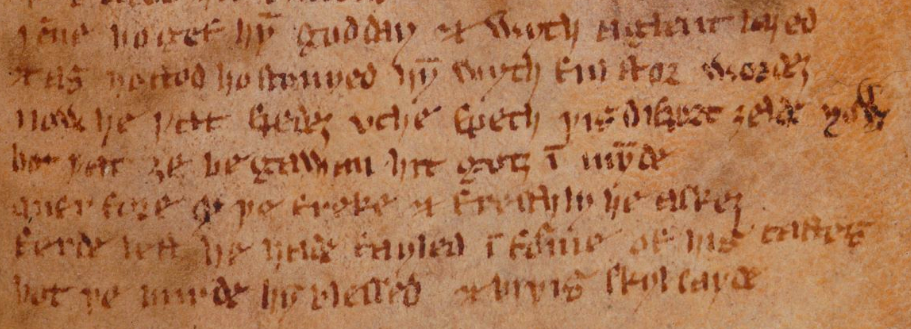
\includegraphics[width=\textwidth]{chapters/img/Gawain.png}
    \caption{\textit{Sir Gawain and the Green Knight}}
    \label{fig:Gawain}
\end{figure}

Although the text samples in this chapter may have seemed a bit alien-looking, the truth is that once we inspect the manuscripts, this effect grows much stronger. In \figref{fig:Gawain}, we show you some of the final lines of one of the sheets of the \textit{Sir Gawain and the Green Knight} manuscript (folio 112 recto, or f. 112r).


\begin{quote}
    1290 þenne ho gef hym godday ⁊ wyth aglent laʒed\\
    1291 ⁊ as hostod ho stonyed hym wyth ful stor wordez\\
    1292 now he þatt spedez vche spech þis disport ʒelde you\\
    1293 bot þatt ʒe be Gawan hit gotz in mynd\\
    1294 querfore quoþ þe freke ⁊ freschly\footnote{This word is particularly difficult to read.} he askez\\
    1295 ferde lest he hade fayled in forme\footnote{Modern editors often interpret this as <fourme>, e.g. \citet{TolkienGordon1967}.} of his castes\\
    1296 bot þe burde hym blessed ⁊ biþis skyl sayde
\end{quote}

\noindent Here are your tasks:
\begin{enumerate}
    \item Can you match any of the words we typed ourselves here to anything in the manuscript? (If so, which ones?)
    \item Try to formulate the reasons why you may be struggling reading the manuscript itself. Be as precise as possible.
    \item Try to transliterate one of the lines above using the letter shapes available to you through your regular keyboard. Put yourself in George and Mí\v{s}a's shoes -- we had to make certain decisions when presenting the Middle English text samples to you. How would you go about picking one way to transliterate your line -- what decisions would you make and why?\is{manuscripts|)}
\end{enumerate}


\end{exercises}

\begin{exercises}{Middle English look-ups}
Let's take a closer look at one of the most famous sentences written in Middle English:

\begin{exe}
    \ex \gll sumer is icumen in\\
    summer is come in\\
    \trans `summer has arrived' 
\end{exe}

\noindent Your task will be very practical here: it's useful to know that Middle English dictionaries\is{dictionaries} exist, and it's useful to try using them. You'll be working with the \textit{Middle English Look-Ups}.\footnote{Available here: \url{https://quod.lib.umich.edu/m/middle-english-dictionary/dictionary}.}
\begin{enumerate}
    \item First, search for ``sumer''. Does the dictionary give you any entries? (Sometimes it doesn't!) If so, the next step is checking if the entry suggested by the dictionary\is{dictionaries} makes sense for your Middle English text. If there are more entries, you simply have to go through them to see which could be the most optimal. (We do make your task much easier by providing you with a translation above.)\footnote{You may be wondering why the dictionary doesn't always give you any entries when looking some words up. There's a fairly good reason for this. Remember that there is a lot of spelling variation\is{orthography} in Middle English, and searching for words in this period therefore comes, sometimes, with the headache of trying out different spelling variants to get an entry that matches your sentence in terms of its meaning. The webpage provides you with more details if you decide to delve into Middle English beyond this book.}
    \item Now do the same for ``icumen''. This time, click on the entry which you deem appropriate. Does it provide you with any useful information? Why and/or why not? 
    \newpage
    \item Can you imagine using this dictionary?\is{dictionaries} Give reasons why and/or why not.
\end{enumerate}


\end{exercises}

\begin{exercises}{Which pronoun?}\label{exercise-ME-pronouns}\is{pronouns|(}

We've seen that there was substantial variation\is{regional variation} in pronoun use during the Middle English period. In this exercise, try to put yourself in the shoes of people from around medieval England and decide which pronoun would be most appropriate!

\begin{enumerate}
    \item A 15th-century woman from the north of England talking about another woman
    \item A 14th-century man addressing his lord directly
    \item A 13th-century man from the south of England talking about a group of people
    \item A 14th-century lord addressing one of his subjects directly
    \item A 14th-century man from the Midlands talking about a group of people
    \item A 14th-century lady addressing a group of her subjects directly
    \item A 13th-century owl\footnote{Talking birds\is{birds} were not uncommon in Middle English literature; see the sample texts in \sectref{ME-fowls} and \sectref{ME-owl}.} talking about itself
    \item A 15th-century woman talking about an unknown or unspecific antecedent
    \item A 14th-century man from the south talking about a woman
\end{enumerate}

\noindent In all examples, the nominative case\is{case} form is what we're looking for.\is{pronouns|)}

\end{exercises}
\largerpage

\begin{exercises}{Chaucer and V2 and V3}\label{exercise-chaucer-V2}\is{word order|(}\is{verb-second|(}

Look at the following clauses from texts by Geoffrey Chaucer.\ia{Chaucer, Geoffrey} The \emph{Treatise on the Astrolabe} was written for his son, Lewis. The \emph{Parson's Tale} is one of the Canterbury Tales.

\begin{exe}
    \ex\label{ex:chaucer-V2-a} ther-for have I geven thee a suffisaunt Astrolabe (\emph{Astrolabe})
    \ex\label{ex:chaucer-V2-b} Thus seyn some auctours (\emph{Astrolabe}; ``some authors'' = new information)\is{information status (given/new)}
    \ex\label{ex:chaucer-V2-c} Alwey he maketh a ``but'' atte laste ende (\emph{Parson's Tale})
    \ex\label{ex:chaucer-V2-d} the amiable tonge is the tree of lyf (\emph{Parson's Tale})
    \ex\label{ex:chaucer-V2-e} in helle hir sighte shal be ful of derknesse (\emph{Parson's Tale; ``her sight'' = given information})\is{information status (given/new)}
    \ex\label{ex:chaucer-V2-f} by the azimut in which he stondeth, maystou\footnote{mayst thou} seen in which partie of the firmament he is (\emph{Astrolabe})
\end{exe}

\noindent Here are your tasks:
\begin{enumerate}
    \item For each clause, state whether it shows a) strict V2 or b) information-structure V2 (IS-V2) word order, or whether c) it's impossible to tell.
    \item Is there a generalization about where you find strict V2 and IS-V2?
    \item If so, why do you think this generalization holds?\is{word order|)}\is{verb-second|)}
\end{enumerate}

\end{exercises}

\begin{exercises}{Guard your wardrobe}\label{exercise-wardrobe}\is{lexical doublets|(}
Look up the Present Day English meaning of the following doublets. What is the key semantic difference, if any? Is this result in any way surprising?
\begin{itemize}
    \item \textit{guardian} vs. \textit{warden}
    \item \textit{garderobe} vs. \textit{wardrobe}
\end{itemize}

\noindent Additional doublets/triplets if you'd like more:
\begin{itemize}
    \item \textit{guard} vs. \textit{ward} (as nouns)
    \item \textit{guaranty} vs. \textit{warranty} vs. \textit{warrant}\is{lexical doublets|)}
\end{itemize}


\end{exercises}

\begin{exercises}{Contrasting Present Day English with Middle English: \textit{The Owl and the Nightingale}}\label{ex-Owl}\is{birds|(}

\chili{}

This exercise involves an extract from \textit{The Owl and the Nightingale} (Early Middle English). Look at the nine expressions in bold and explain how they differ from their Present Day English equivalents. Pay attention to as many differences as possible.

\textit{The Owl and the Nightingale} (ll. 101--142), adopted and adapted from \citet{Cartlidge2001}:\medskip

\noindent
\begin{tabularx}{\textwidth}{lQ}
% \lsptoprule
 Middle English & Present Day English \\
 \midrule
 And Þat oþer ȝer a faukun bredde & And some years ago, a falcon was breeding;\\
 \emph{\textbf{his nest (1)}} noȝt wel he ne bihedde: & and she didn't take good care of \emph{\textbf{her nest: (1)}}\\ 
 Þo hit bicom þat he haȝte, & When it turned out that the falcon had hatched her eggs,\\
 \end{tabularx}
\begin{tabularx}{\textwidth}{lQ}
 \& \emph{\textbf{of his eyre (2)}} \emph{\textbf{briddes wraȝte (3)}}; & and \emph{\textbf{from her eggs (2)}} \emph{\textbf{birds were produced (3)}};\\
 ho broȝte his \emph{\textbf{brides (4)}} \emph{\textbf{mete (5)}}, & she brought her \emph{\textbf{chicks (4)}} \emph{\textbf{some food (5)}},\\
 \emph{\textbf{hit was idon (6)}} ov a loþ[e] [cu]ste. & \emph{\textbf{It was done (6)}} by a horrible farting.\\
 \& \emph{\textbf{nom (7)}} þat fule brid amidde, & she \emph{\textbf{dragged (7)}} that nasty chick from their midst,\\
 \& warp hit of \emph{\textbf{þan wilde bowe (8)}}, & and tossed him out off \emph{\textbf{that wild branch (8)}},\\
 Herbi men segget a bispel, & This illustrates a fable that people tell\\
 þeȝ hit ne bo \emph{\textbf{fuliche (9)}} spel; & though it's not \emph{\textbf{entirely (9)}} a fable;\is{birds|)}\\
%  \lspbottomrule
\end{tabularx}


\end{exercises}

\begin{exercises}{Contrasting Present Day English with Middle English: \textit{Sir Gawain and the Green Knight}}\label{ex-Gawain}

\chili{}

Look at the expressions in bold in the text below and explain how they differ from their Present Day English equivalents. You are expected to comment only on phenomena covered as part of the course.

\noindent
\fittable{
\begin{tabular}{cc}
\lsptoprule
 ME & Present Day English \\
 \midrule
 And \emph{\textbf{þe assaut (1)}} watz sesed at Troye &and \emph{\textbf{the assault (1)}} was ceased at Troy \\ 
 Þe tulk þat þe trammes \emph{\textbf{of tresoun (2)}} &the man that the plots \emph{\textbf{of treason (2)}}\\ 
 \emph{\textbf{Þe trewest on erþe (3)}} &\emph{\textbf{the truest on earth (3)}}\\
 And \emph{\textbf{his highe (4)}} \emph{\textbf{{}kynde (5)}} &and \emph{\textbf{his high (4)}} \emph{\textbf{kin (5)}}\\
 Þat \emph{\textbf{burʒe  he biges (6)}} vpon fyrst &that \emph{\textbf{he builds a castle (6)}} first\\
 \lspbottomrule
\end{tabular}
}

\end{exercises}

\begin{exercises}{Improve these statements}\label{ex-statements-ME}
\noindent What's unfortunate about these statements?
\begin{itemize}
\item ``The Old English <hw> spellings changed to <wh> by the time of Present Day English, resulting in a sound change.''\is{orthography}
\item ``In Middle English, we see the adoption of the pronoun \textit{them}, which has a definite initial dental sound.''\is{pronouns}
\item ``\textit{Perspire} is a completely different word than \textit{sweat} and it is therefore a lexical word.''
\end{itemize}
\end{exercises}


\addsec{Texts}
% \label{me-texts}
\begin{texts}{Caxton, Preface to \emph{Eneydos}}\label{ME-Caxton}

William Caxton,\ia{Caxton, William} who introduced the printing press\is{printing press} to Britain, was acutely conscious of language variation and change. In this text, the 1490 preface to his translation of the \emph{Eneydos} (Virgil's\ia{Virgil} \emph{Aeneid}), he reflects on the diversity of English, using the two plural\is{plurals} forms of the word for `egg' -- the older \emph{eyren} and the newer \emph{egges} -- as an example.\footnote{Transcribed from the manuscript\is{manuscripts} image at \url{https://www.bl.uk/learning/timeline/item126611.html}; accessed April 2020; modern punctuation and paragraph breaks added.}

\begin{textglossed}
  \internallinenumbers*{}
  And certaynly our langage now used varyeth ferre from that whiche was used and spoken whan I was borne: for we Englysshe men ben\marginnote{are} borne under the domynacyon\marginnote{domination; moon} of the mone, which is never stedfaste but ever waverynge, wexynge\marginnote{waxing} one season and waneth \& dyscreaseth another season, and that comyn\marginnote{common} englysshe that is spoken in one shyre\marginnote{shire} varyeth from a nother.

  In so moche that in my dayes happened that certayn marchauntes were in a ship in tamyse\marginnote{Thames} for to have sayled over the see into zelande\marginnote{Zeeland} and for lacke of wynde they taryed atte forlonde\marginnote{foreland (the coast)}, and went to lande for to refreshe them. And one of theym named Sheffelde a mercer\marginnote{textile merchant. Note that at this period the word \textit{meat} referred to food in general, not just meat} cam in to an hows and axed for mete, and specyally he axyd after eggys. And the goode wyf answerde that she coude speke no Frenshe.\il{French} And the marchaunt was angry, for he also coude speke no Frenshe,\il{French} but wolde have hadde egges, and she understode hym not.

  And thenne at laste a nother sayd that he wolde have eyren. Then the good wyf sayd that she understod hym wel. Loo what sholde a man in thyse dayes now wryte, egges or eyren? Certaynly it is harde to playse every man by cause of dyversite \& chaunge of langage.
  %\end{linenumbers}
\end{textglossed}
\end{texts}

\largerpage
\begin{texts}{Paston Letters}
\begin{figure}[H]
    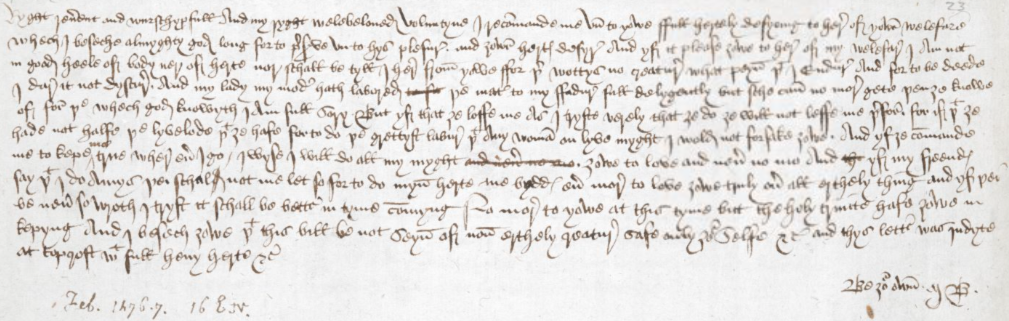
\includegraphics[width=\textwidth]{chapters/img/paston-letter.png}
    \caption{A Paston letter}
    \label{fig:paston}
\end{figure}
The Pastons were a noble family in Norfolk, and we are lucky enough to have many surviving letters to and from members of the family. This letter was written in February 1477 by Margery Paston\ia{Paston, Margery} (née Brews) to her husband John Paston III.\ia{Paston, John}\footnote{Transcribed from the manuscript\is{manuscripts} image in Figure \ref{fig:paston} from \url{http://www.bl.uk/manuscripts/FullDisplay.aspx?ref=Add_MS_43490}, f. 23r; accessed April 2020; modern punctuation and paragraph breaks added.}


\begin{textglossed}
    \internallinenumbers*{}
  Ryght reverent and wurschypfull and my ryght wellbeloved Valentyne, I recomande me unto yowe, ffull hertely desyring to here of yowr wellfare, which I beseche Almyghty God long for to preserve unto his plasyre and yowr hertes desyre.

  And yf it please yow to here of my wellfare I am not in good heele\marginnote{health} of body nor of herte, nor schall be tyll I here from yowe, ffor there wottys\marginnote{knows} no creature what payn that I endure, and for to be deede\marginnote{dead; discover} I dar it not dyscure. And my lady my moder hath labored the mater to my ffadur full delygently, but sche can no more gete than ye knowe of, for the which God knowyth I am full sory.

  But yf that ye loffe me, as I tryste verely\marginnote{verily, i.e. truly} that ye do, ye will not leffe me therefor. For if that ye hade not halfe the lyvelode\marginnote{livelihood} that ye hafe, for to do the grettyst labure that any woman on lyve myght, I wold not forsake yowe. And yf ye comande me to kepe me true wherever I go, I wyse I will do all my myght yowe to love and never no mo.\marginnote{i.e. no one else} And yf my freendys say that I do amyse\marginnote{do amiss, i.e. to make a mistake/go astray}, thei schal not me let so for to do.

  Myne herte me byddys ever more to love yowe truly over all erthely thyng. And yf thei be never so wroth I tryst it schall be better in tyme comyng. No more to yowe at this tyme, but the Holy Trinite hafe yow in kepyng. And I besech yowe that thys bill\marginnote{letter} be not seyne of none erthely creature safe only yorselfe \&c.

  And thys letter was indyte\marginnote{\emph{indyte}: written} at Topcroft with full hevy herte \&c.

  Be\marginnote{by} your own MB.
  %\end{linenumbers}
\end{textglossed}


\end{texts}

\begin{texts}{Sir Gawain and the Green Knight}\label{me-gawain}\is{poetry|(}
\textit{Sir Gawain and the Green Knight} is a chivalric romance from the 14th century. It employs alliteration,\is{alliteration} like Old English poetry, and represents the North West Midland dialect of the Middle English period.\il{Middle English, West Midlands} The following excerpt is a scene in which Lady Bertilak approaches Sir Gawain's bed with romantic intentions in mind. We follow the line numbering of \citet{TolkienGordon1967}.\footnote{Transcribed from the Cotton Manuscript\is{manuscripts} Nero A X/2 from \url{http://www.bl.uk/manuscripts/FullDisplay.aspx?ref=Cotton_MS_Nero_A_X/2&index=4}, ff. 112r-112v; accessed May 2020; original punctuation is kept.}

\begin{textglossed}
  \internallinenumbers*{}
    þenne ho gef hym godday ⁊ wyth aglent laʒed\marginnote{glance; \emph{la\.{ʒ}ed}: smiled}\\
    ⁊ as hostod ho stonyed hym wyth ful stor wordez\marginnote{surprised; \emph{stor}: big}\\
    now he þatt spedez vche spech þis disport ʒelde you\marginnote{\emph{disport}: entertainment}\\
    bot þatt ʒe be Gawan hit gotz in mynd\\
    querfore quoþ þe freke ⁊ freschly\footnote{This word is very difficult to read in the manuscript.\is{manuscripts}} he askez\marginnote{said; \emph{freke}: knight}\\
    ferde lest he hade fayled in forme\footnote{Modern editors often interpret this as <fourme>, e.g. \citet{TolkienGordon1967}.} of his castes\marginnote{afraid; \emph{castes}: speech}\\
    bot þe burde hym blessed ⁊ biþis skyl sayde\marginnote{damsel; \emph{skyl}: reason}\\
    So god as gawayn gaynly is halden\marginnote{\emph{gaynly}: appropriately}\\
    ⁊ cortaysye is closed so clene in hym seluen\\
    couth not lyʒtly haf lenged so long wyth alady\marginnote{\emph{lenged}: stayed}\\
    bot he had craued acusse bihis cõrtaysye\marginnote{\emph{cusse}: kiss; \emph{bihis}: because of his}\\
    bisum towch of summe tryfle at sum talez ende\\
    þen quoþ wowen iwysse worþe as yow lykez\marginnote{\emph{wowen}: Gawain; \emph{iwysse}: indeed}\\
    Ischal kysse at your comaundement as a knyʒt fallez\\
    ⁊ fire lest hedisplese yow fo plede hit no more\marginnote{\emph{fire}: further}\\
    ho comes nerre with þat ⁊ cachez hym in armez\\
    loutez luflych adoun ⁊ þe leude kyssez\marginnote{bends; \emph{leude}: knight}\\
    þay comly bykennen to kryst ayþer oþer\marginnote{\emph{bykennen}: commend}\\
    ho dos hirforth at þe ore with outen dyn more\marginnote{\emph{dyn}: noise}\\
    ⁊ he ryches hym to ryse ⁊ rapes hym sone\marginnote{\emph{rapes}: hastens}\\
    clepes to his chamberlayn choses his wede\marginnote{calls; \emph{wede}: clothes}\\
    boʒez forth quen he watz boun blyþelyto masse\marginnote{turns; \emph{boun}: ready}\\
    ⁊ þenne he meued to his mete þat menskly hym keped\marginnote{\emph{mete}: food; \emph{menskly}: generously}\\
    ⁊ made myry al day til þe mone rysed\\
    with game\footnote{Although this line is usually presented as such in modern editions, it is written as an addition to the previous line in the manuscript\is{manuscripts} itself.}\\
    watz neuer\footnote{These two words are difficult to make out from the manuscript,\is{manuscripts} and we adapt the transcription of \citet{TolkienGordon1967} here.} freke fayrerfonge\marginnote{\emph{fonge}: received}\\
    bitwene two so dyngne dame\marginnote{\emph{dyngne}: worthy}\\
    þe alder ⁊þe ʒonge\\
    much solace setþay same\marginnote{\emph{solace}: joy}
  %\end{linenumbers}
\end{textglossed}


\end{texts}

\begin{texts}{The Reeve's Tale}\label{ME-reeve}
Chaucer's\ia{Chaucer, Geoffrey} \textit{Reeve's Tale} is one of the tales in his \textit{Canterbury Tales}. Below is an extract containing speech between the main protagonists as well as the narrator. They come from different parts of England,\is{regional variation} which we indicate below.\footnote{Taken from \url{https://en.wikisource.org/wiki/Canterbury_Tales_(ed._Skeat)/Reeve}, accessed May 2020; modern punctuation added. For the full version of the Middle English text accompanied with Present Day English interlinear translation, see \url{https://sites.fas.harvard.edu/~chaucer/teachslf/rvt-par.htm}.}

\begin{textglossed}
Aleyn/John (Northern)\il{Middle English, Northern|(}

%   \begin{linenumbers}[4022]
Aleyn \emph{spak} first, ``al hayl, Symond, y-fayth;\\
How \emph{fares} thy faire doghter and thy wyf?''
  %\end{linenumbers}

Miller (Southern)\il{Middle English, Southern|(}

  %\begin{linenumbers}
``Aleyn! welcome,'' quod Simkin, ``by my lyf, \marginnote{\emph{quod}: said}\\
And Iohn also, how now, what do ye heer?'' \marginnote{What are you doing here?}
  %\end{linenumbers}

Aleyn/John (Northern)

  %\begin{linenumbers}
``Symond,'' quod Iohn, ``by god, nede \emph{has} na peer; \marginnote{Need has no peer.}\\
Him \emph{bo\"{e}s} serve him-selve that has \emph{na} swayn, \marginnote{to him has to serve himself that has no servant}\\
Or elles he is a fool, as clerkes sayn.\\
Oure manciple, I hope he wil be deed,\\
\emph{Swa} \emph{werkes} ay the wanges in his heed.\marginnote{aches; always; teeth}\\
And forthy is I come, and eek Alayn, \marginnote{\emph{forthy}: that's why; \emph{eek}: also}\\
To grinde our corn and carie it \emph{ham} agayn;\\ 
I pray yow spede us hethen that ye may.''\marginnote{\emph{hethen}: hence}
  %\end{linenumbers}

Miller (Southern)

  %\begin{linenumbers}
``It \emph{shal} be doon,'' quod Simkin, ``by my fay;\marginnote{\emph{fay}: faith}\\
What wol ye doon whyl that it is in hande?''
  %\end{linenumbers}

Aleyn/John (Northern)

  %\begin{linenumbers}
``By god, right by the hoper wil I stande,''\marginnote{\emph{hoper}: hopper}\\
Quod Iohn, ``and se how that the corn \emph{gas} in;\\
Yet saugh I never, by my fader kin,\\
How that the hoper \emph{wagges} \emph{til and fra}.''
    %\end{linenumbers}

    %\begin{linenumbers}
Aleyn answerde, ``Iohn, and wiltow \emph{swa}?\\
Than wil I be bynethe, by my croun,\\ 
And se how that the mele \emph{falles} doun\\
In-to the trough; that \emph{sal} be my disport.'' \marginnote{\emph{disport}: amusement}
  %\end{linenumbers}

...

Narrator (Southern)

  %\begin{linenumbers}
Whan that he saugh his tyme, softely;\\
He \emph{loketh} up and doun til he \emph{hath} founde\\
The clerkes hors, ther as it stood y-bounde\marginnote{\emph{y-bounde}: tied}\\
Bihinde the mille, under a levesel;\marginnote{\emph{levesel}: arbour}\\
And \emph{to} the hors he \emph{gooth} him faire and wel;\\
He \emph{strepeth} of the brydel right anon.\\
And whan the hors was loos, he \emph{ginneth} gon \marginnote{\emph{ginneth}: begins}\\ 
Toward the fen, ther wilde mares renne,\marginnote{\emph{fen}: marsh}\\
And forth with wehee, thurgh thikke and thurgh thenne.
    %\end{linenumbers}
    
    %\begin{linenumbers}
This miller \emph{gooth} agayn, \emph{no} word he seyde,\\
But \emph{dooth} his note, and with the clerkes pleyde,\\ 
Til that \emph{hir} corn was faire and well y-grounde.
And whan the mele is sakked and y-bounde,\\
This Iohn \emph{goth} out and fynt his hors away,\\
And gan to crye ``harrow'' and ``weylaway''! \marginnote{exclamations of grief}
  %\end{linenumbers}

Aleyn/John (Northern)

  %\begin{linenumbers}
``Oure hors is lorn! Alayn, for goddes \emph{banes}, \marginnote{\emph{lorn}: lost, e.g. forlorn}\\
Step on thy feet, com out, man, al at anes!\\
Allas, our wardeyn has his palfrey lorn.''\marginnote{\emph{palfrey}: saddle horse}
  %\end{linenumbers}

Narrator (Southern)

  %\begin{linenumbers}
This Aleyn al forgat, bothe mele and corn,\\
Al was out of his mynde his housbondrye.
  %\end{linenumbers}

Aleyn/John (Northern)

  %\begin{linenumbers}
``What, \emph{whilk} way is he geen?'' he gan to crye.
    %\end{linenumbers}

...

Aleyn/John (Northern)

    %\begin{linenumbers}
By goddes herte he \emph{sal} \emph{nat} scape us \emph{bathe}.
  %\end{linenumbers}

...

Narrator (Southern)

  %\begin{linenumbers}
And whan the miller saugh that \emph{they} were gon,\\ 
He half a busshel of \emph{hir} flour \emph{hath} take,\\
And bad his wyf go knede it in a cake.
  %\end{linenumbers}

Miller (Southern)

  %\begin{linenumbers}
He seyde, ``I trowe the clerkes were aferd;\marginnote{\emph{trowe}: believe}\\
Yet can a miller make a clerkes berd \marginnote{\emph{berd}: beard}\\
For al his art; now lat \emph{hem} goon \emph{hir} weye.\\ 
Lo where \emph{they} goon, ye, lat the children pleye;\\
\emph{They} gete him \emph{nat} \emph{so} lightly, by my croun!''\marginnote{\emph{gete}: win}
  %\end{linenumbers}
\end{textglossed}\il{Middle English, Northern|)}\il{Middle English, Southern|)}


\end{texts}

\begin{texts}{The Land of Cockaygne}
\textit{The Land of Cockaygne} is a poem written in Irish English\il{English, Irish} of the 14th century. It is one of the so-called \textit{Kildare Poems} (there are sixteen in total). These poems represent our earliest examples of Irish English!\footnote{Not to be confused with \ili{Irish}, i.e. Irish Gaelic, one of the Celtic languages.} As the following extract illustrates, \textit{The Land of Cockaygne} is a piece criticizing the morals of the clergy of the period.\footnote{Transcribed from the Harley 913 Manuscript\is{manuscripts} \url{http://www.bl.uk/manuscripts/Viewer.aspx?ref=harley_ms_913_fs001r}, ff. 3r-3v; accessed May 2020; punctuation kept as in the original. For the full Middle English version, go here: \url{https://celt.ucc.ie//published/E300000-001/}. For a translation into Present Day English, see e.g. \url{http://wpwt.soton.ac.uk/trans/cockaygn/coctrans.htm}.}

\begin{textglossed}
  \internallinenumbers*{}
Fur in see bi west spayngne .\marginnote{\emph{Fur}: far; Spain}\\
is a lond ihote cokaygne ·\marginnote{\emph{ihote}: called}\\
þer nís lond under heuen riche\\
of wel of godnís hit iliche.\marginnote{\emph{iliche}: alike}\\
þoȝ paradis be míri a'bríȝt.\\
cokaygn isof fairír siȝt .\\
what is \.{þ}er in paradis.\\
bot grasse a'flure a'grene ris·\marginnote{\emph{ris}: branches}\\
\.{þ}oȝ \.{þ}er be ioi a'gret dute.\marginnote{\emph{ioi}: joy; \emph{dute}: delight}\\
\.{þ}er nís met bote frute·\marginnote{\emph{met}: food}\\
\.{þ}er nís halle bure no benche·\marginnote{\emph{bure}: bower}\\
bot watír man is þursto qenche·\\
be\.{þ} \.{þ}er no men but two.\\
hely a'enok al so·\marginnote{Elijah and Enoch}\\
clínglich maihi go·\marginnote{dry; may they}\\
whar \.{þ}er woní\.{þ} men nomo·\marginnote{\emph{woní\.{þ}} lives; \emph{men}: indef. ``one''}
  %\end{linenumbers}

  %\begin{linenumbers}
In cokaigne is met A'drínk.\\
wi\.{þ} vte care·how a'swínk.\marginnote{\emph{swínk}: toil}\\
\.{þ}emet is tie·\.{þ}edrínk isclere.\marginnote{\emph{tie}: excellent}\\
to n\'{o}ne· russín a' sopper ·\marginnote{\emph{russín}: snack}\\
i sigge for so\.{þ} boute were·\\
\.{þ}er nís lond on erthe is pere.\marginnote{\emph{pere}: peer}\\
under heuen nís lond iwisse .\\
of so mochil ioi a'blisse·
  %\end{linenumbers}
  
  %\begin{linenumbers}
\.{þ}er is maní swete síȝte·\\
Al is daí nís \.{þ}er no níȝte·\\
\.{þ}er nís baret no\.{þ}er strif ·\marginnote{\emph{baret}: conflict}\\
nís þer no deþ ac euer lif ·\marginnote{\emph{ac}: always}\\
\.{þ}er nís lac of met no clo\.{þ} .\\
\.{þ}er nís man no wōman wro\.{þ} ·\marginnote{\emph{wro\.{þ}}: angry, wroth}\\
\.{þ}er nís serpent wolf no fox .\\
Hors | no capil | kowe· no ox.\marginnote{\emph{capil}: horse, possibly hen}\\
\.{þ}er nís schepe· no swíne no gote.\\
no non horwȝ la godit wote·\marginnote{\emph{horw\.{ȝ}}: dirt; oh god knows it}\\
no\.{þ}er harate nother stode.\\
\.{þ}e lond is ful of o\.{þ}er gode·\\
nís \.{þ}er fleí· fle | no lowse·\marginnote{fly; flee; louse}\\
in clo\.{þ}| in toune· bed no house ·\\
\.{þ}er nís dunnír sl\'{e}te no hawle·\marginnote{thunder; sleet; hail}\\
no non vile worme no snawile ·\\
no non storme| reín, no wínde·\\
Þernís man no wōman blínde .\\
ok al is game Ioií a'gle.\marginnote{\emph{ok}: and}\\
wel is him \.{þ}at þer mai be ·
  %\end{linenumbers}

  %\begin{linenumbers}
Þer be\.{þ} ríuers gret a' fíne ·\\
of oile| melk | honí a' wíne ·\\
watir seruí\.{þ} \.{þ}er to no \.{þ}íng .\\
bot to siȝt a'to wa'ussíng\marginnote{washing}\\
\.{þ}er is maner frute ·\\
Al is solas a' dedute·\marginnote{pleasure; delight}
  %\end{linenumbers}
\end{textglossed}


\end{texts}

\begin{texts}{The Parliament of Fowls}\label{ME-fowls}\is{birds|(}
Chaucer's\ia{Chaucer, Geoffrey} \textit{Parliament of Fowls} (or \textit{Parlement of Foules}) is one of the numerous Middle English works based on ornithology of the times. As the box ``Birds, birds everywhere'' in this chapter (\sectref{ME-meaning}) suggested, there are birds in this piece... and they are all over the place!\footnote{Transcribed from the Harley 7333 Manuscript\is{manuscripts} \url{http://www.bl.uk/manuscripts/Viewer.aspx?ref=harley_ms_7333_fs001r}, ff. 130r--131v; accessed May 2020. For a translation into Present Day English, see e.g. \url{https://medievalit.com/home/echaucer/modern-translations/the-parliament-of-fowls-translation/}.}

\begin{textglossed}
  %\begin{linenumbers}[99]
The were huntere slepyng\textsuperscript{e} in his bed,\marginnote{\emph{were}: weary}\\
To wode a gayne his mynde go\.{þ} a none\\
The juge dremith · how his plees ben spedd,\\
The cartere dremith how his cartis gone\\
The riche of gold · \.{þ}e knyʒt fyʒt with his fone\marginnote{\emph{fone}: foe}\\
The seke met, he drynkth of þe tonne\marginnote{\emph{seke}: sick; \emph{met}: dreams}\\
The louere met he hathe his lady wonne,
  %\end{linenumbers}

...

  %\begin{linenumbers}[183]
A gardyn sa\.{þ} I ful of blosmy bowes\marginnote{\emph{sa\.{þ}}: saw; boughs}\\
Upon a ryver in a grene mede\marginnote{\emph{mede}: meadow}\\
Þere as swetnesse ever y nowy is\\
With\footnote{This word was difficult to decipher and we rely on \citet[386--390]{Benson1991} here.} floures white blewe yalow ⁊ rede\\
And colde welle stremes ⁊ no thing ded,\\
Þat swōm̄yn̄ ful of smale fisshes lyhte\\
W\textsuperscript{t}\marginnote{with} fynnes rede and skales syluer brygte\\
On every bowhe þe bryddes harde I synge\marginnote{bough; birds}\\
W\textsuperscript{t} voyce of aungel in hu· harmonye\marginnote{\emph{hu}: their}\\
Some be syde hem her byrdes forth to brynge\\
The litle conyes to hir pley goŋ hye\marginnote{\emph{conyes}: conies, rabbits}\\
And fer\.{þ}er al aboute I gaŋ aspie\\
Þe dredeful roo · \.{þ}e bukke þe hart ⁊ hynde\marginnote{timid roe; buck; hart; hind}\\
Squerellis · ⁊ bestes smalle\footnote{The manuscript\is{manuscripts} seems to indicate <findlo · ⁊ bethe>, so here we follow \citet[388]{Benson1991} with <· ⁊ bestes smalle>.} of gentil kynde
  %\end{linenumbers}

...

  %\begin{linenumbers}[225]
I sawe bewte · with · oute any A tyre\marginnote{beauty; attire}\\
And yought ful of game ⁊ jolyte\\
ffoule hardines flatery ⁊ desire\\
Messagery and mede ⁊ othir three\marginnote{message-sending; \emph{mede}: bribery}\\
Her names shalle not here, be tolde for me\\
A\'{n}d upōn̄ pilers grete of jaspe longe\\
I Saw A temple of brasse i founded stronge
  %\end{linenumbers}
  
...

  %\begin{linenumbers}[309]
ffor this was on Saint Valantínís daye\\
When every foule comith to chese his mate,\marginnote{\emph{foule}: bird; \emph{chese}: choose}\\
Of every kynde · that meŋ thynk may\\
And that so huge · A noyse gaŋ theí make\marginnote{\emph{ga\.{ŋ}}: began}\\
Þ\textsuperscript{t} Erth ⁊ ere and tree ⁊ every lake\marginnote{\emph{ere}: air}\\
So full was ·\.{þ}\textsuperscript{t} unneth was \.{þ}er space\marginnote{\emph{unneth}: hardly}\\
ffor me to stonde so full was all \.{þ}e place,
  %\end{linenumbers}

...

  %\begin{linenumbers}[323]
That is to sey the foules of ravine\marginnote{birds of prey}\\
were hiest sett ⁊ \.{þ}anne the foules smale\\
Þat etyn as \.{þ}\textsuperscript{t} nature wold enclyne\\
As wormes or \.{þ}ing⁊ of which I tel no tale\\
But water foule satt lowest in the dale\marginnote{\emph{dale}: dale, valley}\\
And foule \.{þ}\textsuperscript{t} liuyth be seed sat on the grene\marginnote{live by seed}\\
And that so fele · \.{þ}at wondir was to sene\marginnote{\emph{fele}: many}
 %\end{linenumbers}
 
 %\begin{linenumbers}[330]
Ther myʒt men \.{þ}e royal Egle fynde\\
That w\textsuperscript{t} his sharpe loke path \.{þ}e sūŋ̄\marginnote{\emph{path}: pierces}\\
And o\.{þ}ere Eglis of a lower kynde\\
Of whiche \.{þ}\textsuperscript{t} clerkes welle devise con̄ū\marginnote{\emph{clerkes}: scholars}\\
Þer was the tirant w\textsuperscript{t} his fetheris don̄\marginnote{\emph{do\.{n}}: dun}̄\\
⁊ grey I mene \.{þ}e goshauke that dothe pyne\marginnote{\emph{goshauke}: goshawk}\\
To bryddis for his outragious ravine\marginnote{\emph{ravine}: greed}
  %\end{linenumbers}

  %\begin{linenumbers}[337]
The gentil faucon̄ that w\textsuperscript{t} his fete distraynith\\
The kyngs honde the hardr sperhauke eke\\
The quaylis foo ·\.{þ}e Emerlion̄ that paynith\marginnote{foe; merlin}\\
Hym selfe ful ofte the larke for to seke\\
Ther was the douve w\textsuperscript{t} hir eyne meke\marginnote{\emph{eyne}: eyes}\\
Þe jelous swān̄ A yens his deth\.{þ}a\textsuperscript{t} syngith\marginnote{\emph{A yens}: against}\\
The Oule eke that of dethe the bode bryngth\marginnote{\emph{bode}: message}
  %\end{linenumbers}

  %\begin{linenumbers}[344]
The crane the geant with his trompes sonne\marginnote{\emph{geant}: giant; sound}\\
The thef the chouwhe · and eke the jangelyng pye\marginnote{chough; magpie}\\
The scornyng jay the Eles fo the heroūn\marginnote{\emph{Eles fo}: eel's foe}̄\\
The fals lapwyng ful of trecherie\\
The stare that the counsel can be wrye\marginnote{starling; betray}\\
The tame ruddok ⁊ the coward kyte\marginnote{\emph{ruddok}: robin}\\
The cok that Orlage is of the thropis lyte\marginnote{\emph{Orlage}: clock;\\\emph{thropis}: village's}
  %\end{linenumbers}

...

  %\begin{linenumbers}[362]
The hote cormeraunt of gloteny\marginnote{\emph{hote}: hot}\\
The ravinwís ⁊ the crowes with hir vois of care\\
The throstell olde \.{þ}e froste feldefare\marginnote{\emph{throstell}: thrush; \emph{feldefare}: fieldfare}\\
What shulde I seyne Of foules every kynde\\
Þat in this world han fetheris ⁊ stature\\
Men myʒt in that place assemble fynde\\
Be fore noble goddes nature\\
And Iche of hem did his besy cure\marginnote{each of them worked diligently}\\
Be nyngly to chese or for to take\\
Be hir acord his formel or his male\marginnote{\emph{formel}: female}
  %\end{linenumbers}
\end{textglossed}


\end{texts}

\largerpage
\begin{texts}{The Owl and the Nightingale}\label{ME-owl}
\textit{The Owl and the Nightingale} is a rare piece, both from a linguistic and a literary point of view. Linguistically, this is a rare sample of early Middle English (13th century). From a literary perspective, the poem presents an altercation type of poetry: the nightingale starts a debate with the owl, arguing about which of the two is the better singer. And if you want to know the answer, you'll have to find the full work and read it!\footnote{Transcribed from the Cotton Caligula A. ix Manuscript\is{manuscripts} \url{http://www.bl.uk/manuscripts/FullDisplay.aspx?ref=Cotton_MS_Caligula_A_IX}, f. 233r; accessed May 2020; punctuation kept as in the original. For the full Middle English version, with a rich commentary, we recommend \citet{Cartlidge2001}.}

\begin{textglossed}
  \internallinenumbers*{}
Ich \.{þ}as ín one sumere dale·\marginnote{\emph{dale}: valley}\\
In one suþe diʒele hale·\marginnote{\emph{suþe}: truly; \emph{diʒele}: secret; \emph{hale}: corner}\\
Iherde ich holde grete tale·\\
An hule and one niʒtingale·\\
Þat plait \.{þ}as stif⁊ starc ⁊strong·\marginnote{\emph{plait}: dispute; strong}\\
Sum \.{þ}ile softe ⁊ lud among.\marginnote{\emph{\.{þ}ile}: while}\\
An aiþer aʒen oþer sval·\marginnote{\emph{sval}: swelled}\\
⁊ let þat vole mod ut al·\marginnote{\emph{vole mod}: foul temper}\\
⁊ eiþer seide of oþeres custe·\marginnote{\emph{custe}: character}\\
Þat alere \.{þ}orste þat hi \.{þ}uste·\marginnote{\emph{\.{þ}orste}: worst; knew}\\
⁊ hure ⁊hure of oþeresonge\marginnote{\emph{hure}: especially}\\
Hi holde plaiding suþe stronge·\marginnote{\emph{plaiding}: pleading}
  %\end{linenumbers}
  
  %\begin{linenumbers}
Þe niʒtingale bigon þe speche·\\
In one hurne of one breche·\marginnote{\emph{hurne}: corner}\\
⁊ sat upone vaire boʒe·\marginnote{\emph{vaire}: fair; \emph{boʒe}: bough}\\
þar \.{þ}ere abute blosme ínoʒe·\\
In ore \.{þ}aste þicke hegge·\marginnote{\emph{ore}: a; \emph{\.{þ}aste}: fast}\\
Imeínd mid spire⁊grene segge·\marginnote{\emph{spire}: reed}\\
Ho \.{þ}as þe gladur uor þe rise·\marginnote{\emph{\.{þ}as}: was; \emph{rise} branch}\\
⁊ song auele cunne \.{þ}íse·\marginnote{in various ways}\\
Bet þuʒte þe dreím þat he \.{þ}ere·\marginnote{\emph{\.{þ}ere}: were}\\
Of harpe ⁊ pipe þan he nere·\marginnote{\emph{nere}: wasn't}\\
Bet þuʒte þat he \.{þ}ere is hote·\marginnote{\emph{is hote}: shot}\\
Of harpe ⁊ pipe þan of þrote·
  %\end{linenumbers}
  
  %\begin{linenumbers}
Þo stod on old stoc þarbiside·\marginnote{\emph{stoc}: stump}\\
Þar þo vle song hire tide·\marginnote{\emph{tide}: canonical hours}\\
⁊ \.{þ}as mid íuí al bigro\.{þ}e·\marginnote{\emph{bigro\.{þ}e}: grown over}\\
Hit \.{þ}as þare hule eardingsto\.{þ}e·\marginnote{\emph{eardingsto\.{þ}e}: abode}\\
Þe niʒtingale hi iseʒ·\\
⁊ hi bihold ⁊ ouerseʒ·\\
⁊ þuʒte \.{þ}el wl of þare hule·\marginnote{\emph{wl}: foul}\\
For me hi halt lodlich ⁊ fule·\marginnote{\emph{lodlich}: loathsome}\\
Vn \.{þ}iʒt ho sede a \.{þ}ei \.{þ}u flo·\marginnote{\emph{Vn \.{þ}iʒt}: monster}\\
Me is \.{þ}e wrs \.{þ}at ich þe so·\\
I \.{þ}is for þine wle lete·\marginnote{foul demeanour}\\
Þel oftich mine song forlete·\marginnote{\emph{forlete}: give up}\\
Min horte atfliþ ⁊falt mitonge·\marginnote{\emph{atfliþ}: flees}\\
Þonne \.{þ}u art tome i\.{þ}runge·\marginnote{\emph{i\.{þ}runge}: thrusted}\\
Me luste bet speten \.{þ}ane singe·\\
Of \.{þ}ine fule ʒeʒlínge·\marginnote{\emph{ʒeʒlínge}: howling\is{birds|)}\is{poetry|)}}
   %\end{linenumbers}
\end{textglossed}


\end{texts}

\begin{texts}{\textit{Ancrene Wisse}}
The following text is an extract from a guide to so-called anchorites or anchoresses. Anchoresses are female hermits -- women who have decided to withdraw from secular society and live in solitude. The text dates back to the 13th century and was written in the West Midlands dialect, possibly not too far from Wales.\footnote{Read more about anchorites and this fascinating Middle English work here: \url{https://d.lib.rochester.edu/teams/text/hasenfratz-ancrene-wisse-introduction}.} But what does \textit{Ancrene Wisse} mean, exactly? Literally, ``anchorites' guide''.\footnote{The following extract is based on the Corpus Christi College MS 402: \url{https://parker.stanford.edu/parker/catalog/zh635rv2202}, f. 13v, our selection corresponds to lines 46--69 in this source \url{https://d.lib.rochester.edu/teams/text/hasenfrantz-ancrene-wisse-part-two}, but for practical reasons, we use our own line numbering and breaks. Accessed December 2021.}

\begin{textglossed}
\internallinenumbers*{}
Lucifer þurh þ\marginnote{\textit{þ}: that} he seh\\
⁊ biheold on him seolf his ahne feiernesse leop in to prude\\
⁊ bicom of angel eatelich\marginnote{\textit{eetelich}: hideous} deouel.\\
Of eue ure alde moder is iyriten\marginnote{\textit{iyriten}: written}\\
on alre earst\marginnote{\textit{earst}: earliest}\\
in hine sunne\marginnote{sin}\\
inȝong\marginnote{\textit{inȝong}: went in} of hire ehsihðe.%\end{linenumbers}

...

%\begin{linenumbers}
þis\marginnote{\textit{þis}: that is} Eue biheold o þe forboden eappel\\
⁊ seh hine feier\marginnote{\textit{feier}: fair, adj.}\\
⁊ feng\marginnote{\textit{feng}: took}\\
to delitin iþe bihaldunge\marginnote{\textit{bihaldunge}: sight}\\
⁊ toc hire lust þer toyard\\
⁊ nom ⁊ et þrof\marginnote{\textit{þrof}: thereof}\\
⁊ ȝef hire laud\marginnote{\textit{laud}: lord}\\
loy\marginnote{\textit{loy}: lo} hu hali yrit spekeð\\
⁊ hu ínyardliche\marginnote{inwardly} hit teleð hu sunne bigon\\
þus eode sunne\footnote{The well-known edited version by Robert Hasenfratz provides as the interpretation of this word \textit{sihthe} instead (\url{https://d.lib.rochester.edu/teams/text/hasenfrantz-ancrene-wisse-part-two}).} biuoren\\
⁊ makede yei\marginnote{way; evil} to uuel lust\\
⁊ com þe dede þrefter\\
þ al moncun\marginnote{mankind}\\ ifeleð\marginnote{feels}%\end{linenumbers}

~

%\begin{linenumbers}
þes eappel leoue suster\\
bitacneð\marginnote{\textit{bitacneð}: represents}\\
alle þe ya\footnote{Hasenfratz translates this as \textit{all the things}.}\marginnote{\textit{ya}: misery}\\
þ lust falleð to\\
⁊ delit\marginnote{delight} of sunne\\
Hyen þu bihaldest te mon,\\
þu art in eue poínt\marginnote{position}.\\
þu lokest oþe\marginnote{\textit{oþe}: on the} eappel.\\
hya se\marginnote{whosoever} hefde iseid to eue\\
þa ha yeorp\marginnote{\textit{yeorp}: cast}\\
earst hire ehe þron\marginnote{\textit{þron}: thereon}:\\
A\marginnote{Ah!; turn} Eue yent te ayei\\
þu yarpest ehe\marginnote{eye; on thy} oþi deað.\\
Hyet hefde ha iondsyeret\marginnote{answered}?\\
Me leoue sire þu hauest yoh\marginnote{\textit{yoh}: wrong}.\\
hyerof chalengest tu me?\\
þe eappel þ ich loki on\\
is forbode me to eotene\\
⁊ nayt\marginnote{\textit{nayt}: not} to bihalden\\
þus yalde{would} Eue inohreaðe\marginnote{enough-readily} habben iondsyeret.\\
O míne leoue sustren\\
as eue haueð monie dehtren þe folhið hare moder\\
þe ondsyerieð o þisse yise\marginnote{in this way}:\\
Me yenest\marginnote{\textit{yenest}: believe} tu\\
seið sum\\
þ ich yulle\marginnote{will, want to} leapen on him\\
þah\marginnote{\textit{þah}: though} ich loki on him?\\
godd yat\marginnote{\textit{yat}: knows} leoue suster\\
mare yunder\marginnote{wonder; happened} ilomp.\\
Eue þi moder leop efter hire ehnen\marginnote{\textit{ehnen}: eyes}.\\
from þe ehe to þe eappel.\\
from þe eappel iparais\marginnote{in paradise}.\\
dun\marginnote{down} to þer eorðe\\
from þe eorðe to helle\\
þer ha\marginnote{\textit{ha}: she} lei\\
i psun\marginnote{\textit{psun}: prison} foyr þusent ȝer ⁊ mare.\\
heo ⁊ hire yere ba \marginnote{\textit{yere}: man; both}\\
⁊ demde\marginnote{\textit{demde}: judged} al hire ofsprung\\
to leapen al efter hire to deað\\
yið uten\marginnote{\textit{yið uten}: without} ende.%\end{linenumbers}

~

%\begin{linenumbers}
Biginnunge ⁊ rote\marginnote{root} of al\\
þis ilke reoyðe\marginnote{same sorrow}.\\
yes aliht sihðe\marginnote{a light}\\
þus often as me\marginnote{\textit{me}: one} seið.\\
of lutel. muchel yaxeð\marginnote{\textit{yaxeð}: grows}.\\
Habbe þenne muche dred euch feble yummon\marginnote{woman}\\
hyen\footnote{Both \textit{hyen} and \textit{hyil} are present in the manuscript\is{manuscripts} as two options.} þeo þe yes riht ta\marginnote{she who was right there; wrought, made; \textit{bisyiken}: deceived}\\
iyraht yið godes honden.\\
Yes þurh a sihðe bisyiken\\
⁊ ibroht in to brad sunne,\\
þet al þe yorld ouerspreadde.
%\end{linenumbers}
\end{textglossed}



\end{texts}

\newpage
\largerpage
\begin{texts}{\textit{Ormulum}}\is{poetry|(}
The \textit{Ormulum} was composed in the East Midlands of England in the twelfth century by a man named Orm\ia{Orm} -- a Norse word meaning ``serpent'', cognate with English \textit{worm}, that was a common Scandinavian name. The text is in verse and uses a unique spelling system:\is{orthography} basically, double consonants\is{consonants} after a vowel show that the preceding vowel\is{vowels} is short. Scholars have argued that the text shows Norse influence not only in the lexicon but also in its syntax \citep{Trips2002}. Norse contact influence is discussed in more detail in \sectref{OE-Scandinavian}, so you may wish to revisit this text once you've read the next chapter. These lines are taken from the edition by \citet{White1878}.



\begin{textglossed}
\internallinenumbers*{}
Adam wass wurrþenn deofless peoww\marginnote{\textit{peoww/þeoww}: slave, servant}\\
Þurrh þatt he dide hiss wille,\\
⁊ all þatt streonedd wass þurrh himm\marginnote{\textit{streonedd}: created, born}\\
Wass streonedd to þatt illke,\\
To ben unnderr deofless þeowwdom,\marginnote{\textit{ben}: be}\\
To farenn all till helle.\marginnote{\textit{faren}: go, travel}\\
⁊ tatt wass rihht tatt mannkinn wass\\
Unnderr þe deofless walde,\marginnote{\textit{walde}: power/rule}\\
All swa summ Adam wurrþenn wass,\marginnote{as Adam had become}\\
Þatt haffde hemm alle streonedd,\\
all se iss her bitwenenn þe\\
⁊ tin eorþlike laferrd;\marginnote{earthly lord}\\
Forr all swa summ þu þeowwtesst himm,\\
Swa shall þin sune himm þeowwtenn,\\
Butt iff he wurrþe lesedd ut\marginnote{\textit{lesedd}: released}\\
Off hiss þeowwdomess bandess.\\
Nu mihht tu sen þatt tatt wass rihht\marginnote{\textit{sen}: see}\\
Þatt mannkinn for till helle,\marginnote{\textit{for}: went}\\
All affterr þatt tatt Adam for,\\ 
Þatt haffde hemm alle streonedd;\\
alle forenn all forrþi\marginnote{\textit{forrþi}: therefore \textit{þeossterrnesse}: darkness}\\
Till helless þeossterrnesse,\\
ȝa þa þatt wærenn gode menn,\marginnote{\textit{ȝa þa ... ȝa þa}: both those ... and those}\\
ȝa þa þatt waerenn ille.\is{poetry|)}
%\end{linenumbers}
\end{textglossed}
\end{texts}



\begin{furtherreading}
A short book-length introduction to the Middle English period in general is \citet{HorobinSmith2002}, and this book also has excellent chapters on the morphology and the lexicon of Middle English. For more on phonology, check out \citet{Minkova2014}, §5.1.3, §5.4, and Chapter 7 in particular. For more on syntax, see \citet[Chapter 4]{Los2015} and \citet{FischerDeSmetvanderWurff2017}. Excepting \citet{Minkova2014}, all these works are written with the student reader in mind.

There are many more diving-off points for specific topics discussed in this chapter. If you're interested in medieval multilingualism,\is{multilingualism} \citet{Davidson2010}, \citet{Hsy2013} and the papers in \citet{JeffersonPutter2013} are good starting points. For pronouns\is{pronouns} and politeness you should try \citet{Burnley2003}. \citet{Sylvester2017} is excellent on the lexicon and semantic change.
\end{furtherreading}
\clearpage
